\documentclass{thesisclass}
% Based on thesisclass.cls of Timo Rohrberg, 2009
% ----------------------------------------------------------------
% Thesis - Main document
% ----------------------------------------------------------------

\usepackage{caption}
\usepackage{blkarray}
\usepackage{framed}
\usepackage{amssymb}
\usepackage{amsmath}
\usepackage[linesnumbered,ruled]{algorithm2e}
\usepackage{graphbox}
\usepackage{multicol}
\usepackage{minted}
\usepackage{etoolbox}
\usepackage{multicol}
\usepackage{colortbl}
\usepackage{wrapfig}
\usepackage{hyperref}
\usepackage{cleveref}
\usepackage{lscape}
\usepackage{mathtools}
\usepackage{todonotes}
\usepackage{multirow}
\usepackage{multirow}
\usepackage{booktabs}
\usepackage{environ}
\usepackage{tabularx}
\usepackage{tikz}
\usepackage{pgf}
\usepackage{tikz-qtree}
\usepackage[acronym,nomain]{glossaries}


%% ---------------------------------
%% | Information about the thesis  |
%% ---------------------------------

\newcommand{\myname}{Rudolf Biczok}
\newcommand{\mytitle}{Integration of internal and external gene expression and drug-perturbation data to empower novel immune therapies against Parkinson’s Disease}
\newcommand{\myinstitute}{Institute of Theoretical Computer Science}

\newcommand{\reviewerone}{Prof. Dr. Alexandros Stamatakis}
\newcommand{\reviewertwo}{Prof. Dr. Ralf Reussner}
\newcommand{\advisor}{Dr. Jitao David Zhang}

\newcommand{\timestart}{1st August 2018}
\newcommand{\timeend}{31st January 2019}

%% -------------------------------
%% |  Information for PDF file   |
%% -------------------------------

\hypersetup{
	pdfauthor={\myname},
	pdftitle={\mytitle},
	pdfsubject={Bioinformatics},
	pdfkeywords={Drug Discovery, Bioinformatics, Data Mining}
}

%% ---------------------------------
%% | Commands                      |
%% ---------------------------------

\DeclareMathOperator{\bin}{bin}
\DeclareMathOperator{\countOp}{count}
\DeclareMathOperator{\ppi}{ppi}
\DeclareMathOperator{\simOp}{sim}
\DeclareMathOperator{\overlap}{overlap}
\DeclareMathOperator{\textToVocs}{text2vocs}
\DeclareMathOperator{\wToV}{w2v}
\DeclareMathOperator{\GO}{GO}
\DeclareMathOperator{\GOD}{GOD}
\DeclareMathOperator{\vecOp}{vec}
\DeclareMathOperator{\wToVSum}{w2vSum}


\newtheorem{definition}{Definition} \numberwithin{definition}{chapter}
\newtheorem{theorem}[definition]{Theorem}
\newtheorem{lemma}[definition]{Lemma}
\newtheorem{corollary}[definition]{Corollary}
\newtheorem{conjecture}[definition]{Conjecture}

\newcolumntype{C}{>{\centering\arraybackslash}X}

\NewEnviron{centeredFigure}[1][]{%
	\begin{figure}[#1]
		\centering
		\BODY
	\end{figure}	
}

\newcommand*\tikzCircled[1]{
	\node[shape=circle,draw,inner sep=2pt, fill=black] (char) {
		\textcolor{white}{#1}
	}
}

\newcommand*\circled[1]{
	\tikz[baseline=(char.base)]{
		\tikzCircled{#1};
	}
}

\newcommand{\thc}[1]{\textbf{\textcolor{white}{#1}}}

\newcommand{\myHeaderCell}[1]{\cellcolor{black}\thc{#1}}

\newcommand{\myMultiLineCell}[2][c]{%
	\begin{tabular}{@{}#1@{}}#2\end{tabular}%
}

\newcommand{\cbrac}[1]{\lbrace #1\rbrace}

%% --------------------------------
%% | Settings for word separation |
%% --------------------------------
% Help for separation:
% In german package the following hints are additionally available:
% "- = Additional separation
% "| = Suppress ligation and possible separation (e.g. Schaf"|fell)
% "~ = Hyphenation without separation (e.g. bergauf und "~ab)
% "= = Hyphenation with separation before and after
% "" = Separation without a hyphenation (e.g. und/""oder)

% Describe separation hints here:
\hyphenation{
% Pro-to-koll-in-stan-zen
% Ma-na-ge-ment  Netz-werk-ele-men-ten
% Netz-werk Netz-werk-re-ser-vie-rung
% Netz-werk-adap-ter Fein-ju-stier-ung
% Da-ten-strom-spe-zi-fi-ka-tion Pa-ket-rumpf
% Kon-troll-in-stanz
}

%Break links in URLs
\def\UrlBreaks{\do\/\do-}


%% ------------------------
%% |    Including files   |
%% ------------------------
% Only files listed here will be included!
% Userful command for partially translating the document (for bug-fixing e.g.)
\includeonly{
titlepage,
chapters/motivation,
chapters/introduction,
chapters/materials,
chapters/results,
chapters/conclusion,
chapters/appendix
}

% Generate the glossary
\makeglossaries

\makeatletter
\renewcommand\listoffigures{%
	\@starttoc{lof}%
}
\renewcommand\listoftables{%
	\@starttoc{lot}%
}
\makeatother

%%%%%%%%%%%%%%%%%%%%%%%%%%%%%%%%%
%% Here, main documents begins %%
%%%%%%%%%%%%%%%%%%%%%%%%%%%%%%%%%
\begin{document}

% Remove the following line for German text
\selectlanguage{english}

\frontmatter
\pagenumbering{roman}
\include{titlepage}
\blankpage

%% -------------------------------
%% |   Statement of Authorship   |
%% -------------------------------

\thispagestyle{plain}

\vspace*{\fill}

\centerline{\textbf Statement of Authorship}

\vspace{0.25cm}

I hereby declare that this document has been composed by myself and describes my own work, unless otherwise acknowledged in the text.

\vspace{2.5cm}

\hspace{0.25cm} Heidelberg, 31st January 2019

\vspace{2cm}

\blankpage

%% -------------------
%% |   Abstract      |
%% -------------------

\thispagestyle{plain}

\begin{addmargin}{0.5cm}

\centerline{\textbf Abstract}

The primary objective of gene set enrichment analysis is to annotate genes of interest with a-priory knowledge in the form of curated gene sets. The problem in this method lies in the large number of reported gene sets and their varying information content. Previous publications suggest to use unsupervised learning methods like hierarchical clustering or self-organized maps to increase interpretability, but there is no metric to assess the quality of these clustering methods or the difference between gene sets itself. We therefore evaluated statistical methods (minkowski, jaccard, kappa-statistic), tree-based methods (gene ontology), network-based methods (shortest path in protein-protein networks), and method based on natural language processing for their capability to measure a biologically plausible distance between gene sets. We used pathway trees from Reactome and a curated tree of immune cell types with corresponding gene sets to benchmark these distance methods.  We found out that document queries with Word Mover's distance on word2vec embedding models yield the best results. \todo{refine based on additional dists}

\vskip 2cm

\centerline{\textbf Deutsche Zusammenfassung}

%Kurze Inhaltsangabe auf deutsch.

\todo{Make german summary at the very end}

\vskip 2cm

\newpage

\centerline{\textbf Acknowledgements}

First and foremost I want to thank the two most valuable point of information Prof Dr. Alexandros Stamatakis and Dr. Jitao David Zhang. The open minded nature of Prof. Stamatakis made this research collaboration possible and his leading expertise in computational bioinformatics tremendously helped us to keep this master thesis in an academic format. Moreover, Dr. Zhang proved his courage and passion in academia by entrusting a theoretical biology research project to an computer science student. His knowledge as principle bioinformatician / biostatistician in an industrial and academic research environment complemented the methodical / computer science expertise of Stamatakis and me beyond expectations.

I send my greetings and thankfulness to Prof. Dr. Ralf H. Reussner, who did not hesitate to take the responsibility as second reviewer. I was a former participant in a two-term research project under the supervision of Prof. Reussner where he demonstrated a high level of methodical knowledge in the engineering aspect of computer science. 

In addition, I want to highlight the support from Gregor Sturm, Sarah Lutteropp, and Lucas Czech\todo{Will lucas be a Dr with the end of this thesis?}. Gregor Sturm is a former master thesis student of Dr. Zhang who shared the curated tree of immune cell types with their respective marker genes. Moreover, he eagerly helped me to extract  all necessary information from his publicly available code repository to save time on my side. Sarah Lutteropp is a PhD student of Prof. Stamatakis and shared her knowledge about methods and limitations in distance-based (phylogenetic) tree inference algorithms. Lucas Czech is also a PhD student under supervision of Prof. Stamatakis and provided me with an implementation skeleton for creating unsupervised clustering algorithms similar to $k$-means in C++.

Although I wish to thank every person in my live who inspired me, helped me, or even influenced my belief system, I must restrict myself to the following group of people that deserve a special place in this section: All members of the HITS Exelixis Lab (Prof. Dr. Alexandros Stamatakis, Dr. Alexey Kozlov, Lucas Czech, Sarah Lutteropp, Pierre Barbera, Benoit Morel, and Ben Bettisworth) and ROCHE BEDA group. Every single member treated me like an equal researcher.

I send my finally thanks and greetings to my parents, who are the only person on earth able to restrain my evil mind and my sister, who happened to be the younger sibling and by extension forced me to be a good role model.

\end{addmargin}

\blankpage

%% -------------------
%% |   Directories   |
%% -------------------

\tableofcontents
\listoftodos
\blankpage

%% -----------------
%% |   Main part   |
%% -----------------

\mainmatter
\pagenumbering{arabic}

%% ==============================
\chapter{Motivation}
\label{ch:motivation}
%% ==============================

\newacronym{rna}{RNA}{Ribonucleic Acid}
\newacronym{dna}{DNA}{Deoxyribonucleic Acid}
\newacronym{ppi}{PPI}{Protein Protein Interactions}

Molecular biology is the aspect of life science thats investigates biological processes on a cellular and molecular level. Biologists in this area seek answers for questions like: ``What is the structural and functional difference between neuron cells compared to other cell types in mammal species?'', ``What influence has chemical compound A when introduced to cell line C?'', or ``Is the cell line derived by following lab protocol A different from the cell line of protocol B?''.
%\begin{wrapfigure}{r}{0.4\textwidth}
%	\centering
%	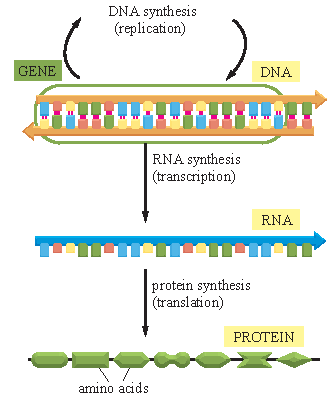
\includegraphics{figures/motivation/central_dogma.pdf}
%	\caption{Central dogma of molecular biology~\cite{citeulike:691434}}
%	\label{fig:central_docma}
%\end{wrapfigure}
%The biggest problem in answering this questions lies within the black-box nature of every living cell. We know that genes play an important role in determine the structure and basic behavior (also known as phenotype) of every organism~\cite{citeulike:691434}. Ongoing research also reveals the functionalities behind each gene ofna n or    
The common procedure to research these questions is to conduct wet lab experiments on prepared cell cultures followed by a computer-assistant gene expression analysis. 
Gene expression is the fundamental biological process of every organism that describes the transcription of \acrfull{rna} from \acrfull{dna} and the translation from \acrshort{rna} to proteins~\cite{citeulike:691434}. 
Collecting and analyzing the gene expression level of every gene inside an organism allows us to identify differentially expressed genes that cause phenotypic differences between cell groups or cell types~\cite{doi:10.1093/bioinformatics/btp616}. To the end, bioinformaticians use public databases of gene sets to see which known cell components or biological processes are reflected by the previously inferred list of differential expressed genes. 
Every gene set represents discovered knowledge in form of name, description and involved genes of a particular biological process. 
Ideally, the entire procedure results in a list of gene sets that uniquely explain the effects of the original wet lab experiment~\cite{doi:10.1093/nar/gks461} (see \cref{sec:gene_expression} for further information about gene expression analysis).

In reality, however, the information gain from reported gene sets is unsatisfying, because 
1) gene sets from even the same database source tend to have a high gene overlap, 
2) gene sets from publicly available databases can have many genes (>200), and 
3) gene set information like title and description can vary in quality depending on the source.
Existing literature suggest supervised learning methods to organize gene sets into a more representative structure. The DAVID algorithm, for instance, performs agglomerative clustering over pairwise kappa statistic between gene sets~\cite{Huang2007}. The authors of this algorithm claim that it maximizes the number of pairwise \acrfull{ppi} within each gene set cluster. However, they also state that it is unclear if this optimization criterion is biologically justified. In general, there exist no gold standard to asses the biological similarity between two gene sets. Having such a gold standard the other hand would make it possible to compare gene set as elements of a metric space. It would enable researchers to benchmark and refine clustering algorithms or to discover new insights from the rapidly growing amount of gene set data.

\section{Own contribution}

We present in this thesis a systematic evaluation of different metrics for pairwise gene set comparisons. We implemented metrics based on 1) statistic methods, 2) gene ontology trees, 3) protein-protein interaction graph networks, and 4) natural language processing methods. For comparing the performance of each distance implementation, we extracted gene sets from data sources whose relationships are already know and preserved as rooted trees. These data sources include 2\todo{update to newest} subsets of the Reactome pathway database~\cite{doi:10.1093/nar/gki072} and a manually curated collection of marker genes for 36\todo{update to newest} human immune cell types~\cite{Sturm463828}. We bundled all distances implementations, data preprocessing, and analysis scripts into a Python package that can be readily extended or included into other algorithms.

Besides gene set analysis, we also spend a significant amount of time building a gen expression analysis framework based on Python. It utilizes a client-server architecture with3 different front-ends for executing and persisting new gene expression experiments (see \cref{sec:roger} for more information).

\section{Structure of this thesis}

The reminder of this document follows the structure of a conventional bioinformatics paper. In \cref{ch:introduction}, we will explain the anatomy of a gene expression analysis pipeline in greater details. In addition, the introduction chapter will cover basic concepts about natural language processing with Word2Vec models and the composition about biological data sources (e.g. gene ontologies, \acrshort{ppi} networks).

\Cref{ch:methods} gives more details about the algorithms behind each implemented metric. We will also summarize the preprocessing steps for the used evaluation data in this chapter.

In \cref{ch:results}, present benchmark results from each metric over the different sets of evaluation date. We will also discuss certain outcome of the results and assess the limitations of different metrics. \todo{Mention the key points here}

And finally, we will draw a final conclusion about our conducted experiments and we will give a future outlook about potential follow-up research in \cref{ch:results}.

%% ==============================
\chapter{Introduction}  \label{ch:introduction}
%% ==============================

%A reader of the introduction should be able to answer the following questions, although not in any depth.
%
%    What is the thesis about?
%    Why is it relevant or important?
%    What are the issues or problems?
%    What is the proposed solution or approach?
%    What can one expect in the rest of the thesis?
%
%State what the thesis is about early. Don't keep the reader guessing until the end of the introduction, or worse, the end of the thesis (don't laugh, I have read draft theses that left me wondering after reading the entire document). You should provide a brief and gentle overview of the thesis topic (or problem) to give the reader enough context  to understand the rest of the introduction. Don't overwhelm the reader with detail at the start. You will provide the details later elsewhere in the thesis. Target the level of writing at one of your peers, but not necessarily somebody working in the same area.
%
%State why the topic is important. Address the "so what?" criteria. Why are you working on the topic? Why should somebody else be interested? Your motivation should be obvious after the introduction, but not necessarily provably so at this point.
%
%State what the major issues are in solving your problem. Coherently overview the issues in enough detail to be able to understand they exist, but don't go into details yet or attempt to prove they exist. The overview should be in just enough depth to understand why you might propose the your particular solution or approach you are taking.
%
%Describe your proposed solution or position you're taking. Again, you should not go into minute details, nor should you attempt to prove your solution at this point; the remainder of the thesis will describe and substantiate your solution in detail, that's what a thesis is :-)
%
%At this point the reader will know what you're working on, why, what are the major issues, and what your proposed solution is, but usually only if he takes your word for it. You should outline what the reader should expect in the rest of the thesis. This is not just the table of contents in sentence form, it is an overview of the remainder of the thesis so the reader knows what to expect. 
%
%
%--------------------------------
%

\section{Gene expression analysis} \label{sec:gene_expression}

\newacronym{rnaseq}{RNA-Seq}{RNA sequencing}
\newacronym{scrnaseq}{scRNA-Seq}{signle cell RNA sequencing}
\newacronym{dge}{DGE}{Differential gene expression}
\newacronym{gse}{GSE}{Gene set enrichment}

Gene set enrichment is the bread and butter of every bioinformatician who tries to discover the genetic reason for phenotypic differences between cell lines. The basic process involves a series of wet and dry lab operations (\cref{fig:gene_expression_analysiss}).

\begin{centeredFigure}[!ht]
	\resizebox{\textwidth}{!}{% <------ Don't forget this %
		\begin{tikzpicture}
			\node[inner sep=0pt] (monocyte1) at (0,0) {
				S1 \enspace \includegraphics[align=c, width=1.1cm]{figures/introduction/macrophage.png}
			};
			\node[inner sep=0pt] (monocyte2) at (0,-1) {
				S2 \enspace \includegraphics[align=c, width=1.1cm]{figures/introduction/macrophage.png}
			};
			\node[inner sep=0pt] (macrophage1) at (0,-2) {
				S3 \enspace \includegraphics[align=c, width=1.1cm]{figures/introduction/microglia.png} 
			};
			\node[inner sep=0pt] (macrophage2) at (0,-3) {
				S4 \enspace \includegraphics[align=c, width=1.1cm]{figures/introduction/microglia.png} 
			};
		
			\node[align=center] (gct) at (6,-1.6) {
				\textbf{Expression data} \\[3pt]
				\setlength\tabcolsep{3pt}
				\begin{tabular}{r|c|c|c|c}
				   	        &    S1  &      S2 & S3 & S4  \\
						\hline
					Sensor 1 &    240 &    415 & 78 & 81 \\
					Sensor 2 &      12 &       4 & 55  & 3  \\
					Sensor 3 &       0 &        0 &        0 &        0  \\
				  	\ldots & \ldots & \ldots & \ldots & \ldots 
				\end{tabular}
			};
		
			\draw [->, ultra thick] (macrophage1.north east) --
				 node [midway,above, align=center] {expression \\ measurement} 
				 node [midway,below, align=center] {microarray, \\ RNA-seq, \\ scRNA-seq, \\ \ldots}
				 (gct);
		
			\node[align=center] (dge) at (13,-1.6) {
				\textbf{DGE top table} \\[3pt]
				\setlength\arrayrulewidth{2pt}
				\setlength\tabcolsep{0pt}
				\arrayrulecolor{white}
				\begin{tabular}{r|c|c|c|c}
					& S1  & S2 & S3 & S4  \\
					\hline
					COL1A1 & \cellcolor{red} & \cellcolor{red!80} & \cellcolor{blue!50} & \cellcolor{blue!20} \\
					\hline
					PLEC & \cellcolor{red!80} & \cellcolor{red!60} & \cellcolor{blue!70} & \cellcolor{blue!50} \\
					\hline
					LOXL4 & \cellcolor{blue!50} & \cellcolor{blue!30} & \cellcolor{red!80} & \cellcolor{red!60} \\
					\ldots & \multicolumn{4}{c}{\ldots} \\
				\end{tabular}
				\arrayrulecolor{black}
			};
		
			\draw [->, ultra thick] (gct) -- 
				node [midway,above] {DGE analysis} 
				node [midway,below, align=center] (dgedesc) {edgeR, \\ DGEseq, \\ limma, \\ \ldots} (dge);
		
			\node[align=left, draw=black, ultra thick, inner sep=3pt,] (gse) at (20.5,-1.6) {
				\textbf{Gene set top table} \\[1em]
				\textit{1. Anchoring fibril formation} \\
				$\left\lbrace COL1A1, COL1A2, \ldots \right\rbrace$ \\[0.5em]
				
				\textit{2. Formation of collagen fibres} \\
				$\left\lbrace LAMA3, LOXL4, \ldots \right\rbrace$ \\[0.5em]
				
				\textit{3. Hemidesmosome formation} \\
				$\left\lbrace PLEC, LAMB3, \ldots \right\rbrace$
			};
		
			\draw [->, ultra thick] (dge) -- 
				node [midway,above] {GSE analysis} 
				node [midway,below, align=center] {CAMERA, \\ \ldots} (gse);
		
			\node[align=right] (fanno) at (5,-6) {
				\textbf{Feature annotation} \\[3pt]
				\setlength\tabcolsep{3pt}s
				\begin{tabular}{r|c|c|c}
					& Symbol & Name& \ldots \\
					\hline
					Sensor 1 & COL1A1 & Collagen type I alpha 1 chain  & \multirow{4}{*}{\vdots} \\
					Sensor 2 & COL1A2 &  Collagen type I alpha 2 chain &  \\
					Sensor 3 & LAMA3 &  Laminin Subunit Alpha 3  &  \\
					\ldots & \ldots & \ldots & \\
				\end{tabular}
			};
		
			\node[align=left] (sanno) at (14.5,-6) {
				\textbf{Sample annotation} \\[3pt]
				\setlength\tabcolsep{3pt}
				\begin{tabular}{r|c|c|c}
					& Cell type & Replication & \ldots  \\
					\hline
					S1 & Macrophage & 1 & \multirow{4}{*}{\vdots} \\
					S2 & Macrophage &  2 &  \\
					S3 & Microglia & 1 & \\
					S4 & Microglia & 2 & \\
				\end{tabular}
			};
		
			\draw [->, ultra thick] (fanno) -- (dgedesc);
		
			\draw [->, ultra thick] (sanno) -- (dgedesc);
		
			\node at (0,1) {\circled{1}};
			\node at (6,1) {\circled{2}};
			\node at (13,1) {\circled{3}};
			\node at (21,1) {\circled{4}};
			
			\node at (5,-4) {\circled{5}};
			\node at (14,-4) {\circled{6}};
		
		\end{tikzpicture}% <------ Don't forget this %
	}
		
	\caption{Gene expression analysis work flow}
	\label{fig:gene_expression_analysiss}
\end{centeredFigure}

At first \circled{1}, a biologist prepares at least two groups of cell lines (generally called samples). The grouping depends on the desired comparison a researcher wants to study, like different immune cell types (e.g. macrophages vs microglia cells~\cite{10.3389/fncel.2013.00045}), healthy cells vs. tumor cells, or perturbed vs. non-perturbed cells. By perturbation we mean any type of cell modification (gene knock-out) or manipulation of the cell environment (e.g. adding drug compounds). It is common practice to cultivate more than one cell line under the same experimental condition (aka. technical replicates) to ensure reproducibility.

The next task describes the generation of gene expression profiles \circled{2}. This involves fixing the cells,  dissolving their membrane, and extracting all \acrshort{rna} fragments. Different methods exist to quantify the \acrshort{rna} concentration per gene and by extension the expression levels. The most frequently used methods are microarray assays, \acrfull{rnaseq}~\cite{citeulike:691434}, and \acrfull{scrnaseq}~\cite{Eberwine2013}. Each method requires different laboratory tasks and computational preprocessing algorithm. The end result of this stage is a table that shows the expression levels for every gene in every sample. The actual meaning of the value can differ depending on the used preprocessing technique. In can, for instance, stand for the total number of \acrshort{rna} fragments counted per gene when using \acrshort{rnaseq}.

After obtaining the raw data, a bioinformatician use linear models to detect genes that are differentially expressed between sample groups \circled{3}. For instance, a widely used software package called edgeR models the entire gene expression experiment as negative binomial distribution to control gene-wise dispersion~\cite{doi:10.1093/bioinformatics/btp616}. The package edgeR uses a variant of the Fisher's exact test to detect \acrfull{dge}. Other packages like limma~\cite{doi:10.1093/nar/gkv007} or DGEseq~\cite{doi:10.1093/bioinformatics/btp612} are flavored depending on the number of technical replicates or used expression measurement technique. 

Experience tells us that genes reported from \acrshort{dge} analysis alone give to view information behind the actual biological phenomena. A single gene can be involved in multiple, partially unknown biological processes or is just an artifact from prior \acrshort{dge} analysis. \acrfull{gse} algorithms try to overcome this issue by using statistical methods and external information about biological processes. One prominent example is implemented in the software package CAMERA~\cite{Wu2012}, which uses competitive gene set tests. The idea behind this competitive tests is to compare every genes inside a gene set relatively to all other genes measured in the experiment. CAMERA in particular uses a modified two-sided $t$-tests capable of detecting inter-gene correlations. The result of this step is a high score \circled{4} of gene sets reflected by the prior list of differentially expressed genes. The content of gene sets used for the \acrshort{gse} is arbitrary and the depends on what sources the bioinformatician choses for analysis. Gene sets from MSigDB~\cite{doi:10.1093/bioinformatics/btr260}, for instance, contains genes that characterize a specific cell type or cell condition. The database Reactome~\cite{doi:10.1093/nar/gki072} on the other hand offers gene sets containing these genes that are part of a particular biological process (aka. pathway).

It is important to note the entire process relies on the existence of feature annotation data \circled{5} and sample annotation data \circled{6}. The feature annotation gives additional information about the measured genes (e.g. name and description of the actual gene that is associated with a particular sensor slot). The sample annotation hold information about origin, and preparation steps for each analyzed cell sample (e.g. cell type, tissue origin, used chemicals).

\section{Pathway \& protein-protein interaction networks}

We can describe every reaction inside or outside a cell as network of protein interactions with organic chemicals, \acrshort{rna}, \acrshort{dna}, or other proteins. \Cref{fig:pathway} illustrates an excerpt of such an interaction network during the mitotic cell cycle.

\begin{centeredFigure}[!ht]
	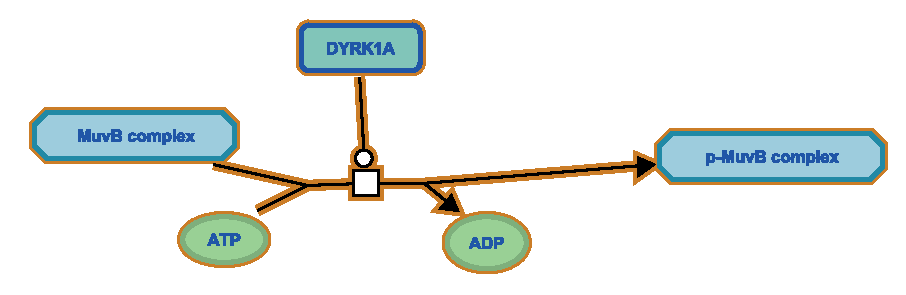
\includegraphics[scale=0.8]{figures/introduction/pathway.pdf}
	\caption[Expert of the mitotic cell cycle.]{Expert of the mitotic cell cycle.  The rectangular boxes and boxes with octagon shape represent proteins. The green nodes represent other organic compounds. The entire pathway involves over different 400 proteins}
	\label{fig:pathway}
\end{centeredFigure}

Public databases like BioGRID~\cite{doi:10.1093/nar/gkw1102} offer a collection of known protein-protein interaction as annotated edge-list. Each edge represents the interaction between one protein with another and hold information about author, detection method, and interaction type. We can use these data sources to compare gene sets in a graph-based representation. It is important to note that not all protein-protein interactions are necessarily part of an actual biological process. This applies for these  protein-protein interactions that researchers discovered outside a cell through regular chemical reaction assay. We use the term pathway to distinguish comprehensive protein-protein interaction networks provided by BioGRID with networks that are known to exist in living cells~\cite{doi:10.1093/nar/gkw1102}.

\section{Gene ontology}

\newacronym{go}{GO}{Gene Ontology}

The \acrfull{go} maintained by the gene ontology consortium~\cite{Ashburner2000,doi:10.1093/nar/gkw1108} is a collection fo controlled vocabulary (aka. \acrshort{go} terms). Every term has is unique identifier (e.g. GO:0030234) and is associated in one of three categories: 1) biological process (e.g. wound healing, epithelial cell proliferation), 2) cellular component (cytoplasm, organelle part), and 3) molecular function (e.g. catalytic activity, enzyme regulator activity). 

\begin{centeredFigure}[!ht]
	\includegraphics[scale=0.4]{figures/introduction/go.png}
	\caption{Excerpt of the gene ontology}
	\label{fig:go}
\end{centeredFigure}

\acrshort{go} terms can have 8 different type of relationships between each other, as seen in \cref{fig:go}. If we only consider the ``is a'' relationships, all \acrshort{go} term of the same category resemble a rooted tree structure. The gene ontology consortium maintains a mapping between \cref{fig:go} terms and gene identifiers, where each \cref{fig:go} term is associated with multiple gene identifiers. In addition, every term carries information origin (as standard evidence code) and function (as unstructured text).

Researcher can use the gene ontology for \acrshort{gse} analysis, where the reported ``gene sets'' are \acrshort{go} terms~\cite{doi:10.1093/bioinformatics/btl140}.  Additionally, algorithms exist to define an arithmetic similarity measurement for \acrshort{go} terms~\cite{doi:10.1093/bioinformatics/btq064}.

\section{Phenotype traits}

\newacronym{embl_ebi}{EMBL-EBI}{European Bioinformatics Institute}
\newacronym{gwas}{GWAS}{Genome-wide association studies}
\newacronym{efo}{EFO}{Experimental Factor Ontology}

Experience shows that the number of observable phenotypes can become unmaintainable depending on the genetic variability of an organism. 
The \acrfull{embl_ebi} provide a controlled vocabulary of traits to characterize phenotypes. 
This vocabulary is called \acrfull{efo} and contains clinical and non-clinical traits. 
A clinical trait represents either a disease (e.g. diabetes type 1) or a disease marker (e.g. measurements of blood glucose concentration). 
Non-clinical traits describe morphological properties that are not disease-related (e.g. exe color). 
Researchers use the standardized phenotype traits to associate diseases or other observable properties with their causing genes. For instance, the \acrfull{gwas} database provides a catalog of manually curated mapping between genes and traits based on findings from over 3000 conducted studies~\cite{doi:10.1093/nar/gkw1133}.
This allows us to compare genes and gene sets based on their prototypical effects in the organisms. \todo{Add excerpt of GWAS}

\section{Natural language processing}

\newacronym{nlp}{NLP}{Natural Language Processing}
\newacronym{bow}{BOW}{Bag Of Words}
\newacronym{wmd}{WMD}{Word Mover's Distance}

According to Wilbur et al. \cite{KIM2017122}, publication databases like PubMed contain over 25 full-text articles with valuable information about biological processes. \acrfull{nlp} techniques like word embeddings opens the opportunity to detect linguistic relationships within unstructured text as it is found in literature databases.

\subsection{Word embedding}

Word embeddings are a class of machine learning models that learn feature vectors from a large set of arbitrary text (aka. text corpus). These feature vectors can be used to project words in a vector space while preserving their semantic similarities. For instance, assume two genes which are part of the same pathway. Then it is likely that the name of the genes appear relatively close to each other in multiple publication. Word embeddings reflect the text distances between the gene names to the feature vector space. Mature examples of world embedding are word2vec techniques, which use feedforward neural as supervised learning method networks~\cite{journals/corr/abs-1301-3781}. 
%\Cref{fig:w2v} shows the two variants of the word2vec model. 

%\begin{centeredFigure}[!ht]
%	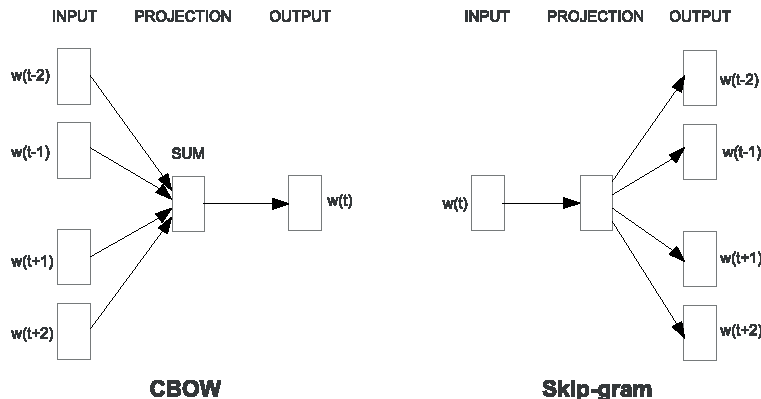
\includegraphics{figures/introduction/word2vec.pdf}
%	\caption{The two variants of the word2vec learning method \cite{journals/corr/abs-1301-3781}}
%	\label{fig:w2v}
%\end{centeredFigure}

\subsection{Document queries}

Inside a vector space, we can use mathematical functions like the euclidean distance or the cosine distance to measure the similarity between single word. However, gene sets consists of multiple genes and can carry additional information like a description or a list of \acrshort{go} terms. One method to compare two sets of words (aka. documents) with each other is word averaging, where the pairwise sum or average of all word vectors build a representation of the document. Kusner et al. claims, however, that ignoring individual word distances could poor comparability between documents that have few words in commin~\cite{Kusner:2015:WED:3045118.3045221}. Other solutions to this problem would be the use of alternative vector representations (e.g. \acrfull{bow}) or more sophisticated distances based on the conventional word vectors (e.g. \acrfull{wmd})~\cite{Kusner:2015:WED:3045118.3045221}. 

%% ==============================
\chapter{Materials and methods} \label{ch:methods}
%% ==============================

Our approach to investigate the similarity between arbitrary gene sets consists of two steps. 
First, we extract reference trees and gene sets from manually curated data sources.
Second, we implement metrics to compare individual gene sets with each other.

\section{Reference data}

\newacronym{ncbi}{NCBI}{National Center for Biotechnology Information}
\newacronym{api}{API}{Application Program Interface}

All used reference trees and gene sets originate from the Reactome database~\cite{doi:10.1093/nar/gki072} and a study conducted by Sturm et al. ~\cite{Sturm463828}. The reference organism in both data sources is the human species.

Evey gene set from Reactome and Sturm et al. contains at least a name and one or more genes. In our reference data, the gene set name has a semantic meaning and describes either the biological process (Reactome) or the cell type (Sturm et al.) reflected by the containing genes.
In general, neither the gene set name nor the type of identifiers used to specify the genes follow a common standard.
Reactome, for instance, uses UniProt identifiers (open protein sequence database)~\cite{doi:10.1093/nar/gkw1099} as primary identifier type for genes. 
However, we can use external annotation services to translate foreign gene identifier types to a preferred one. An example of such an annotation service is Ensembl BioMart~\cite{doi:10.1093/nar/gkx1098}, where a researcher can use the web side or a web service \acrshort{api}. 
Moreover, a gene set curator can assign a gene set with additional information like alternative gene identifiers (e.g. gene symbols alongside to UniProt identifiers) or a description text. The description text contains more details about meaning or origin of the gene set, but is in general unstructured. 
In addition, it is possible to enrich gene sets with information form other sources such as \acrshort{go} terms, gene traits, or any type of unstructured gene description. 

Every used reference trees is rooted and can have inner notes with two or more children. 
Nodes in a reference tree represents exactly one gene set. 
We assume that the reference tree structure resembles the hierarchical relationships between the gene sets. 
This assumption allows us to interpret the tree path lengths between two gene sets as biological distance. 
We therefore consider a metric as biologically plausible if the pairwise distances calculated with the particular metric correlate with the pairwise path lengths.

\subsection{Standard structure} \label{sec:gs_def}

For illustrating the materials and methods used in this work, we define a data point for each gene set as 8-tuple:
\begin{equation} \label{eq:gs_info}
G= \left(G_N, G_{D}, G_{ID}, G_S, G_{GD}, G_{GO}, G_{GOD}, G_{T} \right)
\end{equation}

Each data point consists of the gene set name $G_N$, a gene set description $G_{RD}$, the actual set of genes as \acrshort{ncbi} gene identifiers~\cite{doi:10.1093/nar/gkl993} $G_{ID}$ and gene symbols $G_S$, a set of gene descriptions $G_{GD}$, a multiset of \acrshort{go} terms $G_{GO}$, a multiset of \acrshort{go} term descriptions $G_{GOD}$, and a multiset of phenotype traits $G_{T}$.
\Cref{fig:gs_info} summarizes each element of a data point.
We allow duplication in the multiset elements, because frequency in which formal words appear in data points could influence the similarity between gene sets. 
For instance, data point $G_1$ and $G_2$ can share the same set of \acrshort{go} terms but the number in which each \acrshort{go} terms appear in each data point can still be a differentiating factor.

\begin{table}[!ht]
	\begin{tabularx}{\linewidth}{c|l|X}
		Symbol & Source & Summary \\
		\hline
		$G_N$ & Reactome, Sturm et al. & Gene set name where $G_N \in  \Sigma^*$  \\
		$G_{D}$ & Reactome & Gene set description where $G_{D} \in \Sigma^*$ \\
		$G_S$ & Reactome, Sturm et al. & Set of gene symbols where $G_S \subset \Sigma^*$ \\
		$G_{GD}$& NCBI & Set of gene descriptions $G_{GD} \subset \Sigma^*$\\
		$G_{ID}$ & Reactome, BioMart & Set of NCBI Gene identifiers with $G_{NCBI} \subset L_{NCBI}$ \\
		$G_{GO}$& BioMart & Multiset of \acrshort{go} terms where $G_{GO} \subset L_{GO}$\\
		$G_{GOD}$& BioMart & Multiset of \acrshort{go} term descriptions where $G_{GOD} \subset \Sigma^*$\\
		$G_{T}$ & GWAS & Multiset of phenotype traits with $G_{T} \subset L_{GWAS}$\\
	\end{tabularx}
	\caption{Type of gen set information used in this study.}
	\label{fig:gs_info}
\end{table}

We assume that $G_N$ is a string from the trivial formal language~\cite{Mendelson:2009:IML:1642730} $\Sigma^*$ where $\Sigma$ is the entire ASCII alphabet. 
This assumption also applies to any description $G_D$ provided with the  gene set.
We chose \acrshort{ncbi} as preferred gene identifiers for gene set genes, because Reactome already provide them as alternative to UniProt identifiers. 
In addition, BioGrid uses \acrshort{ncbi} IDs as primary identifiers for their \acrshort{ppi} network data.
$G_{ID}$ is therefore always a subset of $L_{NCBI}$ where the formal language $L_{NCBI} \subset \lbrace 0,\ldots,9 \rbrace^*$ represents all existing \acrshort{ncbi} identifiers. 
Additionally, we collect the gene symbols $G_S$ that correspond to the \acrshort{ncbi} identifiers, where each gene symbol is an element of $\Sigma^*$. 
It is more common to mention genes by their gene symbols in literature and therefore are more likely to appear in word embedding models. 
Moreover, \acrshort{ncbi} offers gene descriptions, which we collect as set $G_{GD}$ for each gene set. 
These gene descriptions can contain information like function, mutations, or pathology of a specific gene as unstructured text (hence $G_{GD} \subset \Sigma^*$).
We used the BioMart annotation web services to collect all \acrshort{go} terms from each \acrshort{ncbi} gene ID as multiset $G_{GO}$. 
All \acrshort{go} terms are part of a standardized collection of identifiers, which we address by $L_{GO} \subset \lbrace GO: \rbrace \cdot \lbrace 0, \ldots, 9 \rbrace^*$. 
In addition, we used BioMart web services to download the term description of each \acrshort{go} term as multiset $G_{GOD}$.
The \acrshort{go} consortium reviews the individual term description, but the descriptions follow neither a standard vocabulary nor a format (i.e., $G_{GOD} \subset \Sigma^*$).
Finally, we used a downloadable database from the \acrshort{gwas} web site to gather all phenotype traits from each gene as multiset $G_T$. 
The phenotype traits are all part of a controlled vocabulary we identify as $L_{GWAS} \subset \Sigma^*$.

\subsection{Reactome reference trees}

\newacronym{tsv}{TSV}{Tab Separated Values}

Reactome is a publicly available database that provides peer-reviewed pathways~\cite{doi:10.1093/nar/gki072}. 
The graph database consists of more than 20 rooted trees where each tree represents a high level activity such as ``Cell Cycle'', ``DNA Repair'', or ``Developmental Biology''.
Each tree contains a hierarchy of pathways that either resemble a sub-activity within a bigger pathway or share a common effect (e.g. ``Disease of Immune System'' and ``Neurodegenerative diseases'' share the effect ``disease'' and are therefore children of pathway ``Disease''). 
Every pathway in Reactome has an unique ID (e.g. R-HSA-1643685), a name, a set of gene with UniProt as primary gene identifier, alternative identifiers like \acrshort{ncbi} gene IDs, and a gene set description as unstructured text. 
The meaning of the description text varies depending on how deep the pathway is located in one of the over 20 pathway trees. In pathway ``Disease'', the descriptions resembles an introducing summary over diseases. In contrast, the descendant pathway ``Binding of SHC1 to p-6Y-EGFR mutants'' describes all actor (genes and other organic molecules), interactions, and references involved in the pathway.

For the evaluation of metrics, we will interpret every (sub) pathway as autonomous gene set. We utilize the following work flow to extract reference trees and data points for a given Reactome ID: 
First, we consume the web service \acrshort{api} from Reactome to download the reference tree and all aforementioned information for each ancestor pathway.
Second, we used the same web \acrshort{api} from Reactome to extract gene identifiers. The primary identifiers are UniProt IDs, but Reactom also offers \acrshort{ncbi} IDs. 
We, however, filtered genes from a pathway if their associated UniProt ID has no corresponding \acrfull{ncbi} IDs.
Third, we removed all ancestor pathways that appear more then once within the reference tree. 
Fourth, we used web services from BioMart, \acrshort{ncbi}, and the data source from \acrfull{gwas} to annotate every gene set with gene descriptions, \acrshort{go} information, and phenotype traits.

\begin{table}[!ht]
	\centering
	\begin{tabular}{l|r|r|r}
		Reactome ID & Tree depth & No. used gene sets & No. removed gene sets \\
		\hline
		R-HSA-1474290 & 4 & 82 & 0 \\
		R-HSA-373755 & 4 & 48 & 0 \\
		R-HSA-8982491 & 5 & 40 & 0 \\
		R-HSA-422475 & 3 & 335 & 1 \\
	\end{tabular}
	\caption{Reactome pathways used as reference trees.}
	\label{fig:reactome_trees}
\end{table}

\subsection{Immune cell differentiation hierarchy}

All cells of the human immune system descend from a common progenitor immune cell.
Progenitor cells are specialized stem cells with the ability to differentiate into a dedicated set of cell types.
It is possible to identify differentiation state and function of an immune cell by its so called marker genes. 
Marker genes are genes whose expression levels give evidence to a specific cell function or state. 
Gregor et al.~\cite{Sturm463828} utilize this knowledge to evaluate cell-type quantification methods. 
They investigated the prediction accuracy of algorithms that quantify the fraction of cell types in any given tissue sample.
For the evaluation process, Gregor et al. conducted a literature research to curate a hierarchy of 45 cell types.
In addition, they collected a set of marker gene symbols for 38 of the 45 cell types if they are backed up by previous studies.
Gregor et al. provide the cell type hierarchy and the marker genes as downloadable \acrfull{tsv} documents on a public source repository~\cite{Sturm463828}. 

For our analysis, we interpreted the cell types with their individual set of marker genes as gene sets and the cell type hierarchy as reference tree. We performed the following preprocessing steps on the raw data: 
First, we excluded 5 of 45 cell types that neither have any child cell types with marker genes nor carry marker genes themselves.
Second, we performed a post-order traversal of the reference tree to calculate missing sets of marker genes for the inner nodes of the cell type tree.
For each inner node without marker genes, we calculate the union over all marker genes set that are direct children of the particular inner node. 
This is in our opinion reasonable, because pathways in Reactome are always a supersets of their child pathways.
Third, we removed 4 of 40 cell types that are cancer cells, because we are unsure if cancer cell provide stable marker genes. This filtering step leaves us with 36 out of 45 immune cell types. \todo{We may want to run experiments on these cells as well}
Fourth, we used BioMart to translate gene symbols into \acrshort{ncbi} gene identifiers. In addition, we used BioMart and the other annotation services mentioned in \cref{sec:gs_def} to obtain data points. An illustration of the immune cell reference tree is in \cref{fig:immune_cell_tree}.

\begin{centeredFigure}[!ht]
	\resizebox{\textwidth}{!}{% <------ Don't forget this %
		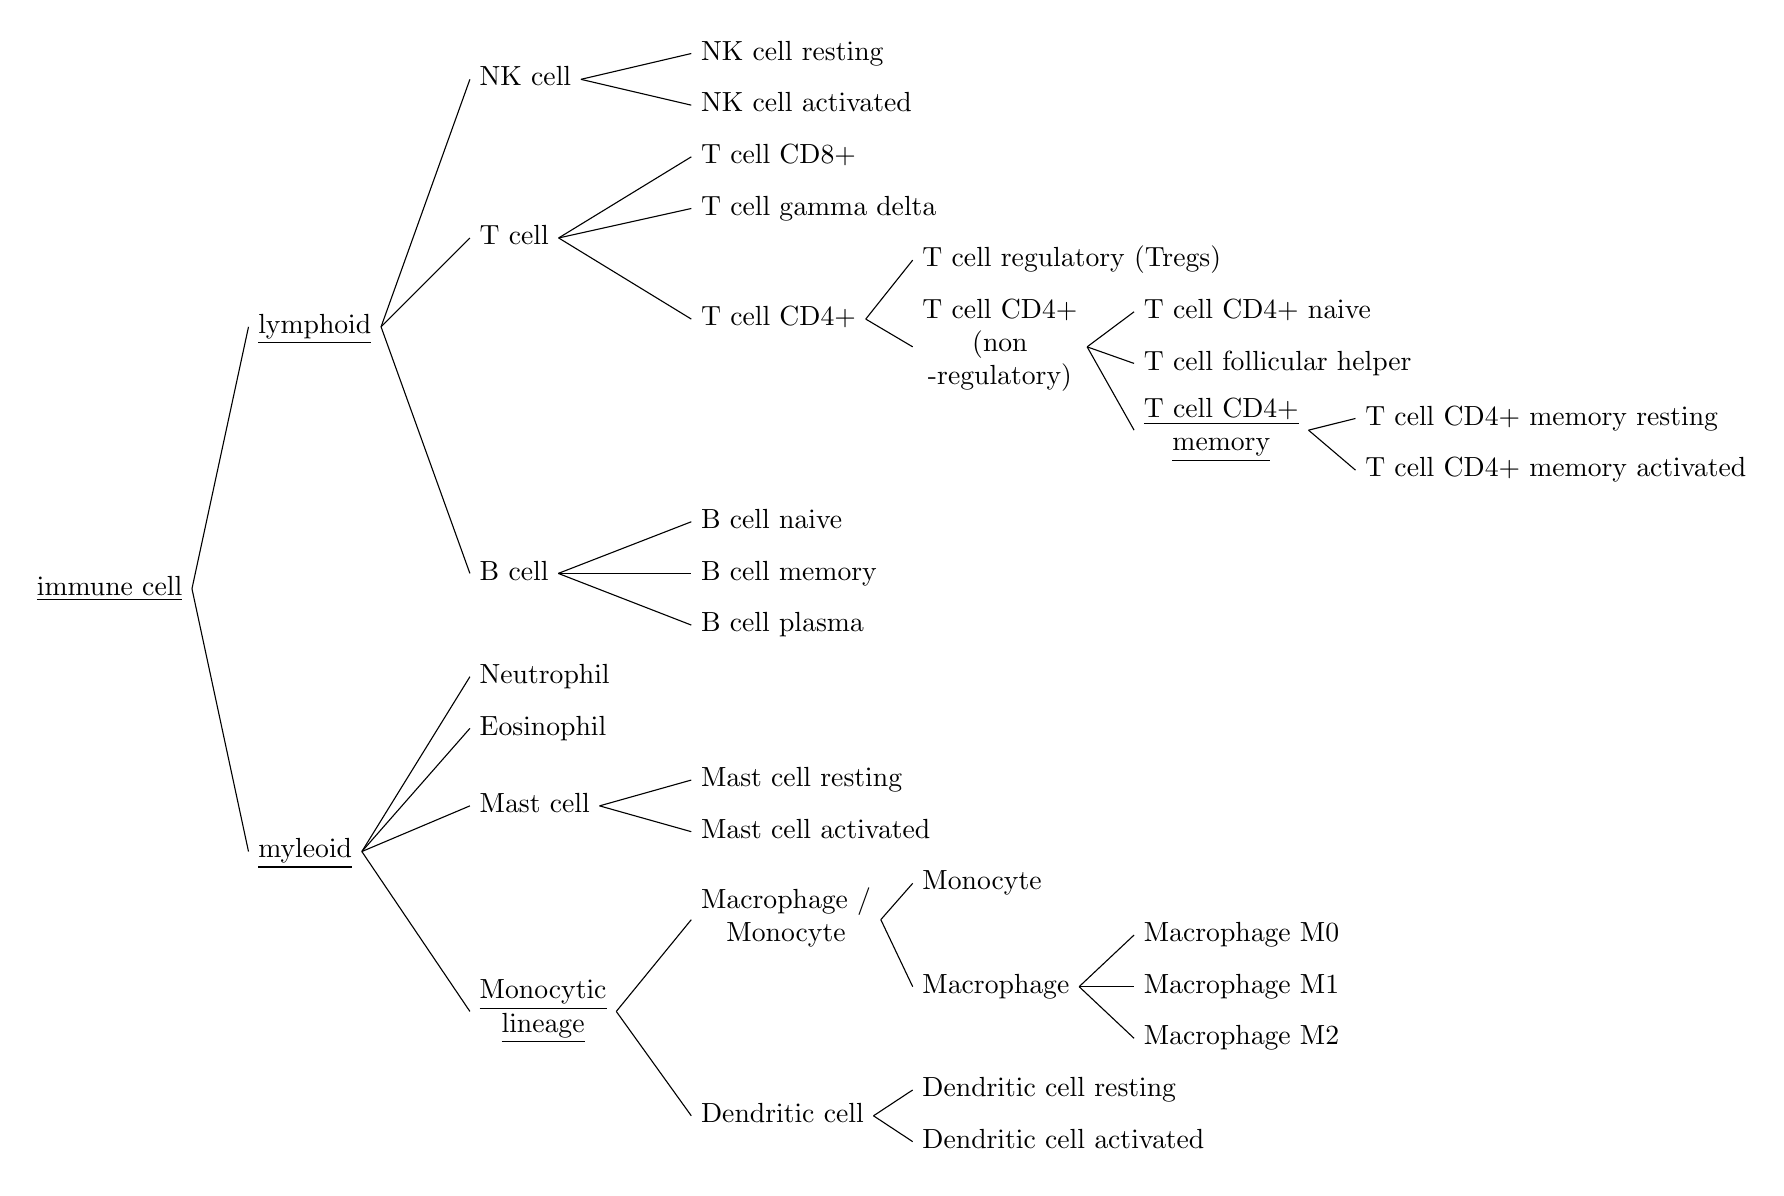
\begin{tikzpicture}[sibling distance=0pt]
		\tikzset{grow'=right,level distance=80pt}
		\tikzset{execute at begin node=\strut}
		\tikzset{every tree node/.style={align=center,anchor=base west}}
		\Tree[.{\underline{immune cell}}
		   [.{\underline{lymphoid}}
		      [.{NK cell}
		         \text{NK cell resting}
		         \text{NK cell activated} ]
		      [.{T cell}
		         \text{T cell CD8+}
		         \text{T cell gamma delta}
		         [.{T cell CD4+}
		            \text{T cell regulatory (Tregs)}
		            [.{T cell CD4+\\(non\\-regulatory)}
		               \text{T cell CD4+ naive}
		               \text{T cell follicular helper}
		               [.{\underline{T cell CD4+}\\\underline{memory}}
		                  \text{T cell CD4+ memory resting}
		                  \text{T cell CD4+ memory activated} ] ] ] ]
		      [.{B cell}
		         \text{B cell naive}
		         \text{B cell memory}
		         \text{B cell plasma} ] ]
		   [.{\underline{myleoid}}
		      \text{Neutrophil}
		      \text{Eosinophil}
		      [.{Mast cell}
		         \text{Mast cell resting}
		         \text{Mast cell activated} ]
		      [.{\underline{Monocytic} \\ \underline{lineage}}
		         [.{Macrophage /\\Monocyte}
		            \text{Monocyte}
		            [.{Macrophage}
		               \text{Macrophage M0}
		               \text{Macrophage M1}
		               \text{Macrophage M2} ] ]
		         [.{Dendritic cell}
		            \text{Dendritic cell resting}
		            \text{Dendritic cell activated} ] ] ] ]
		\end{tikzpicture}% <------ Don't forget this %
	}

	\caption[Immune cell type tree used as referenc.]{Immune cell type tree used as reference. Data from Georg et al.  does not provide marker genes for the underlined cell types}
	\label{fig:immune_cell_tree}
\end{centeredFigure}

\section{Gene Set Metrics}

Let $\mathcal{G}$ be the universe of all data points $G$ that follow the 8-tuple schema for gene sets in \cref{eq:gs_info}. We assume that all data points in $\mathcal{G}$ are organized in a rooted tree according to their biological relationship. Furthermore, let $l_{\mathcal{G}}(G_1, G_2)$ be the path length between $G_1$, $G_2 \in \mathcal{G}$ within this tree. Our goal is to find a mathematical metric~\cite{Arkhangel} $d: \mathcal{G} \times \mathcal{G}  \to [0, \infty)$ so that $d(X, Y)$ and $l_{\mathcal{G}}(X, Y)$ are statistical depended for any random variable $X$ and $Y$.

Every gene set metric we present has two degrees of freedom: A projection $p : \mathcal{G} \to X$ and a distance function $D: X \times X \to [0, \infty)$ over a set $X$. The operator $D$ performs the actual statistical or algorithmic calculation where $p$ projects a data point from $G \in \mathcal{G}$ to a mathematically controlled space $X$. We use the set $\mathcal{A}  = \lbrace{N,D, ID, S,GO, GOD, GD,T \rbrace}$ to address an specific element of data point $G \in \mathcal{G}$.

Moreover, we will use the following nomenclature to distinguish presented metrics from each other:
\begin{align} \label{eq:metric_def}
	\begin{split}
		d_{p, D} \colon \mathcal{G} \times \mathcal{G} & \to [0, \infty) \\
		(G_1,G_2) & \mapsto D \left( t(G_1), t(G_2) \right).
	\end{split}
\end{align}
\Cref{fig:metrics} shows a list of all metrics used in this work.

\begin{table}[!ht]
	\centering
	\begin{tabularx}{\linewidth}{l|X}
		\hline
		Metric & Description \\
		\hline
		\multicolumn{2}{l}{Statistical metrics} \\
		\hline
		$\displaystyle d_{P_{ID}, D_J}$ & Jaccard distance over \acrshort{ncbi} gene identifiers $G_{ID}$\\
		$\displaystyle d_{P_{T}, D_J}$ & Jaccard distance over gene traits $G_T$ \\
		$\displaystyle d_{P_{ID}, D_O}$ & Overlap distance over \acrshort{ncbi} gene identifiers $G_{ID}$\\
		$\displaystyle d_{P_{T}, D_O}$ & Overlap distance over gene traits $G_T$ \\
		\hline
	    $\displaystyle d_{\bin_{ID}, D_{p=1}}$ & Manhattan distance over \acrshort{ncbi} gene identifiers $G_{ID}$ \\
	    $\displaystyle d_{\bin_{T}, D_{p=1}}$ & Manhattan distance over gene traits $G_T$ \\
		$\displaystyle d_{\countOp_{T}, D_{p=1}}$ & Manhattan distance over gene trait counts \\
		$\displaystyle d_{\bin_{ID}, D_{p=2}}$ & Euclidean distance over \acrshort{ncbi} gene identifiers  $G_{ID}$\\
		$\displaystyle d_{\bin_{T}, D_{p=2}}$ & Euclidean distance over gene traits $G_T$ \\
		$\displaystyle d_{\countOp_{T}, D_{p=2}}$ & Euclidean distance over gene trait counts \\
		$\displaystyle d_{\bin_{ID}, D_\kappa}$ & $\kappa$ distance over \acrshort{ncbi} gene identifiers $G_{ID}$\\
		$\displaystyle d_{\bin_{T}, D_\kappa}$ & $\kappa$ distance over gene traits $G_T$ \\
		$\displaystyle d_{\countOp_{T}, D_C}$ & Cosine distance over gene trait counts \\
		\hline
		\multicolumn{2}{l}{Graph-based metrics} \\
		\hline
		$\displaystyle d_{GO_{BP}, D_{Wang,BMA}}$ & Wang method over \acrshort{go} terms (biological process terms) \\
		$\displaystyle d_{GO_{CC}, D_{Wang,BMA}}$ & Wang method over \acrshort{go} terms (cellular component terms) \\
		$\displaystyle d_{GO_{MF}, D_{Wang,BMA}}$ & Wang method over \acrshort{go} terms (molecular function terms) \\
		$\displaystyle d_{GO_{BP}, D_{Resnik,BMA}}$ & Resnik method over \acrshort{go} terms (biological process terms) \\
		$\displaystyle d_{GO_{CC}, D_{Resnik,BMA}}$ & Resnik method over \acrshort{go} terms (cellular component terms) \\
		$\displaystyle d_{GO_{MF}, D_{Resnik,BMA}}$ & Resnik method over \acrshort{go} terms (molecular function terms) \\
		\hline
		$\displaystyle d_{P_{ID}, D_{Dijkstra,BMA}}$ & Dijkstra method over \acrshort{ncbi} gene identifiers in \acrshort{ppi} networks \\
		$\displaystyle d_{N_{ppi}, D_J}$ & Jaccard distance over direct neighbor \acrshort{ncbi} gene identifiers in \acrshort{ppi} networks \\
		$\displaystyle d_{N_{ppi}, D_O}$ & Overlap distance over direct neighbor \acrshort{ncbi} gene identifiers in \acrshort{ppi} networks \\
		\hline
		\multicolumn{2}{l}{Word embedding metrics} \\
		\hline
		$\displaystyle d_{\wToVSum \circ\ P_{S},D_C}$ & Cosine distance over word vectors of gene symbols $G_S$  \\
		$\displaystyle d_{\wToVSum \circ\ P_{D}, D_C}$ & Cosine distance over word vectors of descriptions $G_D$  \\
		$\displaystyle d_{\wToVSum \circ\ P_{GD}, D_C}$ & Cosine distance over word vectors of gene descriptions $G_{GD}$  \\
		$\displaystyle d_{\wToVSum \circ\ GOD_{BP}, D_C}$ & Cosine distance over word vectors of \acrfull{go} terms (biological process)  \\
		$\displaystyle d_{\wToVSum \circ\ GOD_{CC}, D_C}$ & Cosine distance over word vectors of \acrfull{go} terms (cellular components) \\
		$\displaystyle d_{\wToVSum \circ\ GOD_{MF}, D_C}$ & Cosine distance over word vectors of \acrfull{go} terms (molecular function) \\
		$\displaystyle d_{\wToV \circ\ P_{S}, D_{WM}}$ & Word Mover's distance over word vectors of gene symbols $G_S$  \\
		$\displaystyle d_{\wToV \circ\ P_{D}, D_{WM}}$ & Word Mover's distance over word vectors of descriptions $G_D$  \\
		%$\displaystyle d_{\wToV \circ\ P_{GD}, D_{WM}}$ & Word Mover's distance over word vectors of gene descriptions $G_{GD}$  \\
		%$\displaystyle d_{\wToV \circ\ GOD_{BP}, D_{WM}}$ & Word Mover's distance over word vectors of \acrfull{go} terms (biological process)  \\
		%$\displaystyle d_{\wToV \circ\ GOD_{CC}, D_{WM}}$ & Word Mover's distance over word vectors of \acrfull{go} terms (cellular components) \\
		%$\displaystyle d_{\wToV \circ\ GOD_{MF}, D_{WM}}$ & Word Mover's distance over word vectors of \acrfull{go} descriptions (molecular function) \\
		\hline
	\end{tabularx}
	\caption{Implemented gene sets metrics.}
	\label{fig:metrics}
\end{table}

\subsection{Statistical metrics}

We define a gene set metric as statistical metric if it does not rely on external topologies such as trees, networks or word embeddings. Moreover, we identify two subgroups of statistical methods: 1) set-based metrics (e.g., over Jaccard coefficient, and overlap coefficient) and 2) vector-space-based metrics (e.g., Minkowski distance, cosine distance, and distance based on $\kappa$ coefficient).

For set-based methods, we define the trivial projection $P_A$ that selects an attribute from the data point $G$ as follows:
\begin{align} \label{eq:trivial_projection}
	\begin{split}
		P_A : \mathcal{G} & \to \mathcal{P}(\Sigma^*) \\
		G & \mapsto  G_A,
	\end{split} \qquad A \in \mathcal{A} = \lbrace{ N,D, ID, S,GO, GOD, GD,T \rbrace}
\end{align}
This allows us to explicitly state which information of the gene set we want to use for defining metrics.
We used the Jaccard index $J$ and the overlap coefficient~\cite{Vijaymeena} to define corresponding distance functions:
\begin{align}
	D_J(A,B) = 1-J(A,B) =\begin{dcases}
			0 & \text{if } A=B=\emptyset \\
			1 - \frac{\left| A \cap B \right|}{\left| A \cup B \right|}  &\text{else}.
		\end{dcases}
\end{align}
\begin{align}
	D_O(A,B) = 1- \overlap(A,B) = \begin{dcases}
					0 & \text{if } A=B=\emptyset \\
					1 - \frac{\left| A \cap B \right|}{\min(\left| A \right|, \left| B \right|)} &\text{else}.
				\end{dcases}
\end{align}
Both distances generate values between 0 and 1, where 0 represents perfect overlap. in contrast to $D_J(A,B)$, $D_O(A,B)$ will always return 0 if one of the two arguments is a subset of the other argument.

For vector-space-based gene set metrics, let $\mathcal{G}_A = \bigcup_{G_i \in \mathcal{G}} P_A(G_i)$ be the set of formal words that appear in at least one data point $G \in \mathcal{G}$ when looking at attribute $A \in \mathcal{A}$.
We can then project $G \in \mathcal{G}$ as binary vector in $\mathbb{R}^n$, $n =  \left| \mathcal{G}_A \right| $ by the following function:
\begin{align} \label{eq:bin}
	\begin{split}
		\bin_A \colon \mathcal{G} & \to \mathbb{R}^n \\
		G^A & \mapsto x \text{ such that } x_j = \begin{cases}
			1 \iff w_j \in P_A(G_i) \\
			0 \qquad else
		\end{cases}\text{for all } j \in \left\lbrace 1, \ldots,  n \right\rbrace, w_j \in\mathcal{G}^A.
	\end{split}
\end{align}
For example, the $j$-th entry in $\bin_{ID}(G)$, is $1$ if the $j$-th \acrshort{ncbi} gene identifier is present in data point $G$.

As mentioned in \cref{sec:gs_def}, we purposely allow duplicates for certain gene set information (i.e., \acrshort{go} terms, \acrshort{go} descriptions, and phenotype traits). 
We therefore introduce a transformation $\countOp_A$ that assigns every data point $G \in \mathcal{G}$ to a counts vector $f \in \mathbb{R}^n$ with $n =  \left| \mathcal{G}_A \right|$: 
\begin{align} \label{eq:count}
	\begin{split}
		\countOp_A \colon \mathcal{G} & \to \mathbb{R}^n \\
		G_A & \mapsto f \text{ such that } f_j = \left| \lbrace w \in G_A: w = w_j \rbrace \right|  \text{for all } j \in \left\lbrace 1, \ldots,  n \right\rbrace, w_j \in\mathcal{G}_A.
	\end{split}
\end{align}

The Minkowski distance~\cite{treves2006topological} describes a class of mathematical distances over $\mathbb{R}^n$, $n \in \mathbb{N}$ and is defined as
\begin{align} \label{eq:minkowski_dist}
	D_p(x,y) = \begin{dcases}
		\left( \sum_{i=1}^{n} |x_i-y_i|^p\right)^{\frac{1}{p}} & \text{if } p \in [1,\infty) \\
		\max_{i \in \lbrace 1, \ldots n \rbrace} |x_i-y_i| &\text{if } p = \infty.
	\end{dcases} \qquad \forall x, y \in \mathbb{R}^n
\end{align}
The $k$-means clustering algorithm, for instance, uses the Euclidean distance ($p=2$), for measuring the error between centroids and assigned vectors.

The cosine distance~\cite{Vijaymeena} is defined as
\begin{equation} \label{eq:cosine_dist}
	D_C(x,y)= 1- \frac{x \cdot y}{\left\| x \right\| \left\| y \right\|} \qquad \forall x, y \in \mathbb{R}^n
\end{equation}
where $x \cdot y$ is Euclidean dot product between $x$ and $y$. It is the preferred operator to measure the distance between word embedding vectors.

The $\kappa$ coefficient $\kappa$ measures the agreement between two classifiers~\cite{Artstein:2008:IAC:1479202.1479206}. Its general form is defined as:
\begin{align*} \label{eq:kappa}
	\kappa = \frac{p_0-p_e}{1-p_e}, \quad p_e = \frac{1}{N^2} \sum_{k} n_{k,1} n_{k,2}, \quad \kappa \in [-1, 1]
\end{align*}
Where $p_0$ is the agreement between the two classifiers relative to the number of $N$ observations and $p_e$ is the probability that the two classifier agree by chance. The factors $n_{ki}$ represent the number of times where classifier $i \in \lbrace 1,2 \rbrace$ predicts category $k$.
If the classifiers have total agreement with each other, the resulting $\kappa$ coefficient is 1.
A $\kappa$ coefficient of 0 or below implies total disagreement or classification performance worse than random selection.
If we interpret gene sets as binary classifiers (e.g. classifiers for gene symbols), we can utilize the $\kappa$ coefficient as distance operator for $x$, $y \in \mathbb{R}^n$:
\begin{equation} \label{eq:kappa_dist}
	D_\kappa(x, y)= 1-\kappa(x, y) = \frac{1-p_0(x,y)}{1-p_e(x,y)} \quad 
	\begin{array}{l}
		\displaystyle p_0(x,y) = \frac{c_1(x,y)+ c_0(x,y)}{n} \\
		\displaystyle p_e(x,y) = \frac{n_0(x)n_0(y)+ n_1(x)n_1(y)}{n^2}	
	\end{array}
\end{equation}
Where $n_k(v)$ is the number of entries in vector $v \in \mathbb{R}^n$ that have value $k$, and $c_k(v_1,v_2)$ the number of times where both vector $v_1$ and $v_2$ have value $k$ at position $i \in \lbrace 1, \ldots, n\rbrace$.

We implemented the statistical gene set metrics by using Python software packages scikit-learn~\cite{scikit-learn} for the $\kappa$ coefficient and SciPy~\cite{scipy} for Jaccard intex, cosine similarity, and Minkowski distances.

\subsection{Graph-based metrics}

\newacronym{dag}{DAG}{Directed Acyclic Graphs}
\newacronym{bma}{BMA}{Best Match Average}

For graph-based gene set metrics, we require an additional data structure that models relationships between data point attributes (like \acrshort{ncbi} gene IDs $G_{ID}$) as a mathematical graph. 
We distinguish between methods that assume a \acrfull{dag} (e.g. gene ontologies) and methods that operate on arbitrary graphs (e.g. protein-protein interaction networks).
We incorporated the Resnik similarity~\cite{Resnik:1999:SST:3013545.3013547} and the Wang similarity~\cite{Wang:2007:NMM:1346066.1346071} as basis for the \acrshort{dag}-based distances $D_{Wang,BMA}$ and $D_{Resnik,BMA}$.
Both Resnik and Wang propose their similarity functions for comparing the similarity between two individual \acrshort{go} terms. Furthermore, we used the Dijkstra algorithm~\cite{Cormen:2009:IAT:1614191} to measure the path lengths between two individual genes in a \acrshort{ppi} network ($D_{Dijkstra, BMA}$). For each of the three methods, we apply the \acrfull{bma} strategy~\cite{Pesquita} to combine the results of pairwise comparison. Moreover, we define projections for \acrshort{go} information that filters terms based on their category (e.g., $GO_{BP}$ for selected only terms that describe a biological process). Finally, the $N_{ppi}$ projection extends a set of \acrshort{ncbi} gene identifiers by its direct neighbors in the \acrshort{ppi} network.

Let $DAG_{GO} = (L_{GO}, E_{GO})$ be the \acrshort{dag} over all \acrshort{go} terms $L_{GO}$ where $E_{GO}$ represents the \acrshort{go} term relationships as tuple.
Furthermore, let $C_t$ be the set that contains all descendant terms of \acrshort{go} term $t \in L_{GO}$ and $t$ itself. 
The Resnik similarity is then defined as
\begin{align*}
	\begin{split}
		\simOp_{Resnik} : L_{GO} \times L_{GO} & \to[0,1]\\
		(t_1, t_2) & \mapsto IC(LCA(t_1, t_2)),
	\end{split} 
	\quad IC(t) = - \log \left(  \frac{|C_t|}{|L_{GO}|} \right),
\end{align*}
where $LCA(t_1,t_2)$ is the lowest common ancestors of the \acrshort{go} terms $t_1$, $t_2$. 
The function $IC(t)$ describes the information content of term $t$ relative to the entire ontology. 
Two \acrshort{go} terms are similar in the context of Resnik similarity, if their lowest common ancestor selects a relatively small portion of the gene ontology. We define the corresponding Resnik distance as $D_{Resnik}(t) = 1- \simOp_{Resnik}(t)$ for every \acrfull{go} term $t$.

For the Wang similarity, let $T_t$ be the set that includes all ancestors of $t$ and $t$ itself. The following function then calculates the Wang similarity
\begin{align*}
	\begin{split}
		\simOp_{Wang} : L_{GO} \times L_{GO} & \to[0,1]\\
		(t_1, t_2) & \mapsto \frac{\displaystyle \sum_{t\in T_{t_1} \cap T_{t_2}} \left(S_{t_1}(t)+ S_{t_2}(t) \right) }{SV(t_1)+SV(t_2)},
	\end{split}.
\end{align*} 
Where $S_t(t')$ is the semantic contribution of $t'$ to the ancestor $t$ and $SA(t)$ the sum of all semantic contributions over all ancestors of $t$:
\begin{align*}
	S_t(t') & = \begin{dcases}
			1   & \text{if } t' = t \\
			\max \lbrace w_e \cdot S_t(c)\colon c \text{ is children of } t' \rbrace & \text{else}
	\end{dcases}, \quad SV(t) = \sum_{t' \in T_t} S_t(t'),
\end{align*}
The factor $w_e$ is called semantic contribution of edge $e$ in $E_{GO}$. Wang suggest to assign constant values to semantic contribution factors based on the relation type of the edges (e.g., ``is-a'', ``regulates'', \ldots).
We define the corresponding Wang distance as $D_{Wang}(t) = 1- \simOp_{Wang}(t)$ for every \acrfull{go} term $t$.

The comparison of two (multi)sets of \acrshort{go} terms requires an additional combination strategy. 
Let $GO_1$, $GO_2$ be subsets of $ L_{GO}$ and $D_f$ a distance function for individual terms (e.g. $D_{Resnik}, D_{Wang}$). 
The  \acrshort{bma} strategy then calculates the distance between two \acrfull{go} term multisets by the following expression:
\begin{align*}
		D_{f,BMA}(GO_1, GO_2) & =  \frac{\displaystyle \sum_{t_1\in GO_1} \min_{t_2 \in GO_2} D_f(t_1,t_2) +  \sum_{t_2 \in GO_2} \min_{t_1 \in GO_1} D_f(t_1,t_2)}{|GO_1| + |GO_2|}.
\end{align*}
The function $D_{Wang,BMA}$, for instance, computes the Wang distance over two sets of terms by using the \acrshort{bma} combination strategy. An important property of the \acrshort{bma} strategy is that the identity-of-indiscernibles property for distances functions holds if $D_f$ is a distance function (i.e., $d(x,y) = 0 \iff x=y$). 

Moreover, one can generalize the \acrshort{bma} strategy for an arbitrary distance function $D_f$ that operates on elements from an arbitrary set. 
We use the \acrshort{bma} strategy in combination with the Dijkstra algorithm to define a gene set metric over \acrshort{ppi} networks ($D_{Dijkstra,BMA}$). 
The Dijkstra algorithm uses a greedy approach to find the shortest path between two nodes. 
In the context of \acrshort{ppi} networks, the input nodes resemble \acrshort{ncbi} gene identifiers from a data point $G$.

Next, we define projections for extracting \acrfull{go} terms from data points of a certain category.
The tree \acrfull{go} categories are ``Biological Process'' (BP), ``Cellular Component'' (CC), and ``Molecular Function'' (MF), wich also represent the tree root terms for all other \acrshort{go} terms.
We use $L_{GO_{BF}}$, $L_{GO_{CC}}$, $L_{GO_{MF}}$ to differentiate between \acrshort{go} term of different categories, i.e. $L_{GO_{BF}} \cup L_{GO_{BF}} \cup L_{GO_{BF}} = L_{GO}$. We do this analogously for \acrshort{go} term descriptions $L_{GOD_{BF}}$, $L_{GOD_{BF}}$, and $L_{GOD_{BF}}$.
Furthermore, we define projections for ontology terms $GO_X$  and ontology term descriptions $GOD_X$ as:
\begin{align} \label{eq:ontology_projection}
	\begin{split}
		GO_X : \mathcal{G} & \to \mathcal{P}(L_{GO_X}) \\
		G & \mapsto P_{GO}(G) \cap L_{GO_X},
	\end{split} \qquad X \in \lbrace{ BP, MF, CC \rbrace}
\end{align}
\begin{align} \label{eq:ontology_desc_projection}
	\begin{split}
		GOD_X : \mathcal{G} & \to \mathcal{P}(L_{GOD_X}) \\
		G & \mapsto P_{GOD}(G) \cap L_{GOD_X},
	\end{split} \qquad X \in \lbrace{ BP, MF, CC \rbrace}
\end{align}
This separation is necessary, because we want to see how important the \acrshort{go} category is during the distance evaluation phase. In addition, the Resnik method does not support comparison with mixes \acrshort{go} terms.

Finally, we define the $N_{ppi}$ projection as 
\begin{align} \label{eq:ppi_neighbours}
	\begin{split}
		N_{ppi} : \mathcal{G} & \to \mathcal{P}(L_{NCBI}) \\
		G & \mapsto P_{ID}(G) \cup \{g' \in L_{NCBI}\ |\ \exists g \in P_{ID}(G) : \{g, g'\} \in E_{PPI} \},
	\end{split}
\end{align}
where $E_{PPI}$ contains the edges of a given \acrshort{ppi} network.

The tab-delimited data we used for the \acrshort{ppi} network originate from the BioGRID~\cite{doi:10.1093/nar/gkw1102} homepage. We extracted the edges as tuple of \acrshort{ncbi} identifiers from each row and filtered edges that did not originate from homo sapiens. We used an implementation of the Dijkstra algorithm provided by the SciPy package as base for the Dijkstra distance function. The R package GOSemSim~\cite{doi:10.1093/bioinformatics/btq064} offered the implementations for the Resnik similarity and the Wang similarity. In addition, we used the R data package org.Hs.eg.db~\cite{goAnno}, which includes the relationships between \acrshort{go} terms for the human species. 

\subsection{Word embedding metrics}

The two crucial parts of the presented word embedding metrics are 1) the embedding model and 2) the functions to project gene set information into the word2vec vector space.
Additionally, we included the \acrshort{wmd} as specialized mathematical distance for the word embedding vector spaces.

For explaining the Word2vec model and the projection function, we need to clarify the difference between formal words and natural language words. 
A formal word is an element of a formal language  $L \subset \Sigma^*$ over an alphabet $\Sigma$ and can contain every character. On the contrary, a word in the context of natural language consists only of printable characters. We use the term ``vocable'' to distinguish formal words from natural language words.
In a trained Word2vec model $M \in \mathbb{R}^{v \times d}$, we represent every vocable by a $d$-dimensional row vector in $M$ where $v$ is the size of the model vocabulary.
Our reference Word2vec model is a pretrained model provided by Wilbur et al.~\cite{KIM2017122}. 
They extracted over 25 million titles and abstracts from publications in PubMed (until March 2016). 
\todo{Link to dataset?} 
%https://www.ncbi.nlm.nih.gov/CBBresearch/Wilbur/IRET/DATASET/
Wilbur et al. trained the model with the skip-gram variant of the Word2vec learning method.

As mentioned in the previous section, we cannot project formal words directly into the word vector space.
It is therefore necessary to extract usable vocables from formal words / arbitrary text. 
For our evaluation, we conducted the following steps for each formal word:
First, we replace every upper case character by a lower case character. This is necessary because our reference model is only trained for lower case vocables.
Second, we split each formal word by any kind of word divider (dot, coma, colon, semicolon, whitespace, tabulator, slash, hyphen, brackets) and obtain a list of vocables.
Third, we remove numbers and out-of-vocabulary elements from the split list.
Finally, we remove stopwords based on the English language. Stopwords represent a set of frequently used vocables in a language that don't add significant value to a list of vocables (e.g. ``the'' or ``of'' in the English language).

With this preprocessing steps in mind, we define the transformation of an arbitrary subset of a formal language into a (mult)iset of vocables:
\begin{equation*}
		\wToV :  \mathcal{P}(\Sigma^*) \to \mathcal{P}(\Sigma^*), \quad W \mapsto \bigcup_{w \in W}  \textToVocs(w),
\end{equation*}
where $\textToVocs$ performs the previously mentioned preprocessing steps for each formal word. 
Furthermore, we define
\begin{equation*}
		\wToVSum :  \mathcal{P}(\Sigma^*) \to \mathbb{R}^d, \quad W \mapsto \sum_{v \in  \wToV(W)} \vecOp(v) ,
\end{equation*}
as sum of all vocables extracted for a given set of formal words. The expression $\vecOp(v)$ returns the vector representation of the vocable $v$. 
The $\wToVSum$ allows us to build projections from gene set date points into word embedding as composition with other projection function. 
For instance, we use the composition $\wToVSum \circ P_{S}$ to denote the transformation of gene symbols into word vectors. Note that Word2vec generally ignores the order of words, which makes it unnecessary to preserve the order of vocables from the input set.

Existing mathematical distance functions over $\mathbb{R}^d$, like the cosine distance $D_C$, are suitable for building gene set metrics. Alternatively, we can use functions like the \acrfull{wmd}~ \cite{Kusner:2015:WED:3045118.3045221}, which are more suited for document-based queries. 
In the context of \acrshort{wmd}, we use the term ``document'' as synonym for (multi)sets of words. 
The \acrshort{wmd} distance takes two documents and calculates the document distances based on the optimal pairwise pairing of vocables (see \cref{fig:wmd}).
\begin{centeredFigure}[!ht]
	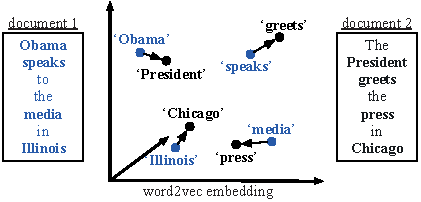
\includegraphics{figures/materials/wmd.pdf}
	\caption{Illustration of WMD distance of two documents~\cite{Kusner:2015:WED:3045118.3045221}}
	\label{fig:wmd}
\end{centeredFigure}
\todo{Expand description?}

We implemented the word-embedding-based gene set metrics by using the Python packages Gensim~\cite{rehurek_lrec} and NLTK~\cite{Loper:2002:NNL:1118108.1118117}. Gensim is a widely used software package for training Word2vec models, performing common Word embedding operations, and performing document queries with \acrshort{wmd}. The NLTK package offers utility functions for downloading English stopwords.

% Signal Transduction 3000

%% ==============================
\chapter{Results \& Discussion}
\label{ch:results}
%% ==============================

We evaluate all presented gene set metrics by assessing the correlation of pairwise distance values with pairwise path lengths per gene set data point. We found out that gene set metrics based on the overlap distance yields the best results in 4 out of 5 Reactome and immune cell tree reference datasets. We were able to detect moderate correlation (absolute correlation value $> 0.5$) in all but one reference datasets. All reference dataset show at least week correlation (absolute correlation value $> 0.3$) for at least one gene set metric.

\section{Ground-truth comparison}

We assume that the reference tree path lengths between gene sets represent the ground truth. 
To compare path lengths with metric results, we calculate distance matrices for each reference dataset $\mathcal{G}$.
A distance matrix is a symmetric matrix $M \in \mathbb{R}^{n \times n}$ where $n$ is the number of gene set data points in the reference data.
Each element $M_{ij}$ contains the pairwise distance $d_{p, D}(g_i,g_j)$ where $g_i$, $g_j$ are gene set data points from  $\mathcal{G}$ and $d_{p, D}$ is one of the presented gene set metrics. 
The symmetry property and the identity-of-indiscernibles property of distance functions allows us to ignore calculations for the lower triangle and the main diagonal of the distance matrix (as seen in \cref{eq:dm})
\begin{equation} \label{eq:dm}
   M = \left(
   \begin{array}{ccccc}
    \cline{1-1}
    \multicolumn{1}{c|}{0} &                  M_{12}     &                        M_{13} & \ldots                                  & M_{1n} \\ \cline{2-2}
                                   &  \multicolumn{1}{c|}{0} &                        M_{13} & \ldots                                  & M_{2n} \\  \cline{3-3}
                                    &                                  & \multicolumn{1}{c|}{0} & \ddots                                 & \vdots  \\ \cline{4-4}
                                    &                                   &                                  &  \multicolumn{1}{c|}{\ddots} & M_{n-1,n} \\ \cline{5-5}
                                    &                                   &                                  &                                             & \multicolumn{1}{c|}{0} \\ 
  \end{array}\right)
\end{equation}

\newacronym{pcc}{PCC}{Pearson Correlation Coefficient}
\newacronym{srcc}{SRCC}{Spearman's Rank Correlation Coefficient}

The evaluation process against the ground-truth consists of 3 major steps.
First, we calculate the distance matrix of pairwise path lengths between gene sets. 
We repeat this for all reference datasets. 
Second, we calculate the distance matrix for a given gene set matrix $d_{p,D}$ over a given reference data set.
We repeat this step for every distance metric and for every reference dataset.
Third, we perform correlation coefficient calculations between gene set metrics and the pairwise path lengths.

At the end of the third step, we have two correlation matrices $C^{P}$ and $C^S$ for each reference dataset.
The matrix entries $C^P_{d_i,d_j}$ stands for the \acrfull{pcc}~\cite{doi:10.1002/9781119454205.ch10} between the distance matrix values calculated by gene set metrics $d_i$, $d_j$ or the reference tree path length. 
Analogously, the matrix entries $C^S_{d_i,d_j}$ represent the \acrfull{srcc}~\cite{doi:10.1002/9781119454205.ch10} between two gene set metrics $d_i$, $d_j$ or a gene set metric and the reference path lengths. 
Researcher use the \acrfull{pcc} to measure the linear dependence between two observable variable. 
The \acrshort{srcc} assesses the monotonic relationship between two variables. Both correlation types have a value range between -1 and 1, where a correlation value near -1 or 1 implies stronger linear or monotonic dependence than a correlation value near 0. 
To be more precise, we distinguish between 4 correlation levels:
\begin{itemize}
	\item No correlation if correlation value is in $(-0.3, 0.3)$
	\item Weak correlation if correlation value is in $(-0.5,-0.3]$ or $[0.3,0.5)$
	\item Moderate correlation if correlation value is in $(-0.9,-0.5]$ or $[0.5,0.9)$
	\item Strong correlation if correlation value is in $[-1.0,-0.9]$ or $[0.9,1.0]$
\end{itemize}

\Cref{fig:pearson} illustrates an excerpt of the $C^P$ matrix. 
It shows only the correlation values between gene set metrics and the pairwise path lengths merged from all reference datasets. 

\begin{centeredFigure}[!ht]
	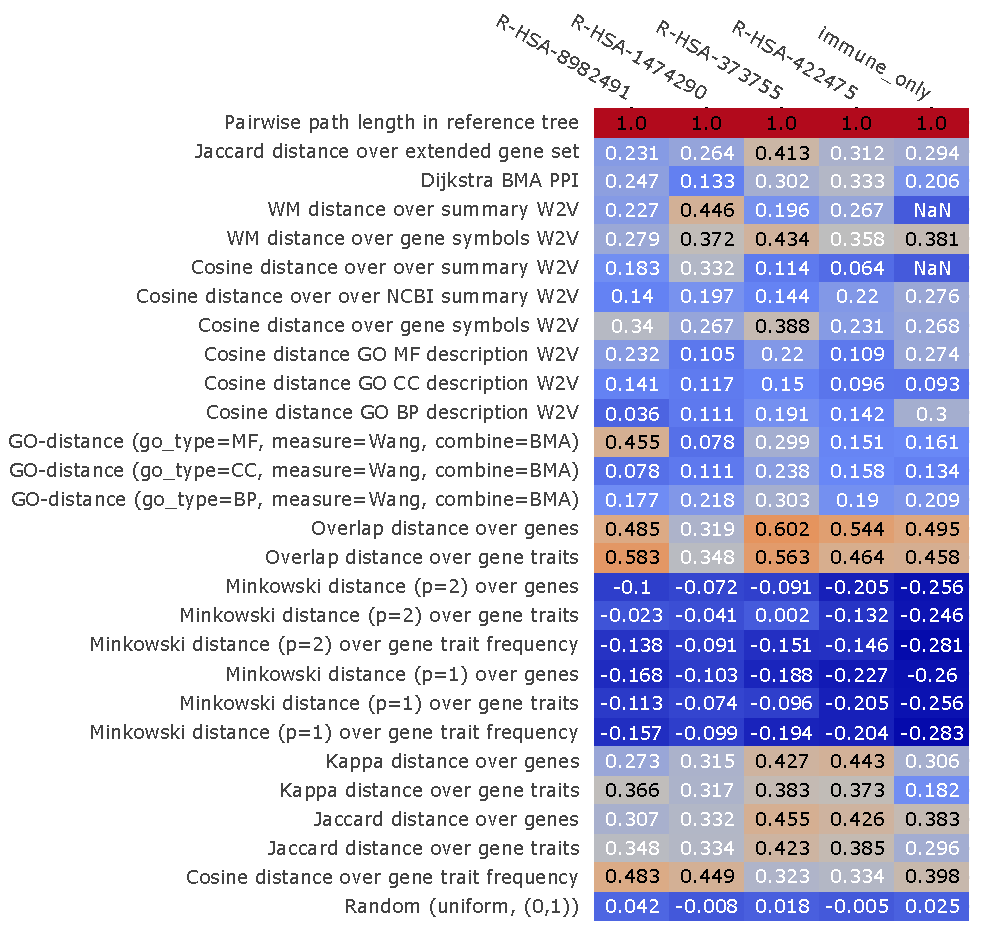
\includegraphics[scale=0.85]{figures/results/plots/summary/pearson.pdf}
	\caption[Pearson correlation between gene set metrics and path lengths]{Pearson correlation between gene set metrics and path lengths. The reason for NaN values in the immune cell dataset is the lack of gene set descriptions from the raw data}
	\label{fig:pearson}
\end{centeredFigure}

The majority of the presented gene set metrics, including a random baseline, show  at best weak correlation.
This especially applies to metrics that uses Minkowski functions as mathematical distance.
Other statistical metrics, however, perform better compared to graph-based metrics and metrics that uses word embeddings.
The overlap distance in particular has the highest correlation values among all reference data sets except the Reactome subtree ``R-HSA-1474290''.
In dataset ``R-HSA-1474290'', we see that the \acrshort{wmd} distances and cosine distance over gene count vectors show the highest correlations.

The \acrshort{srcc} values in \Cref{fig:spearman} support our finding that statistical metrics outperform more sophisticated gene set metrics based on graphs or word embeddings. Especially gene set metrics that uses the overlap distances function show moderate correlation levels. 
Furthermore, we see that gene identifiers and phenotype traits are enough to achieve moderate correlation where other external gene set annotations don't improve correlation.

\begin{centeredFigure}[!ht]
	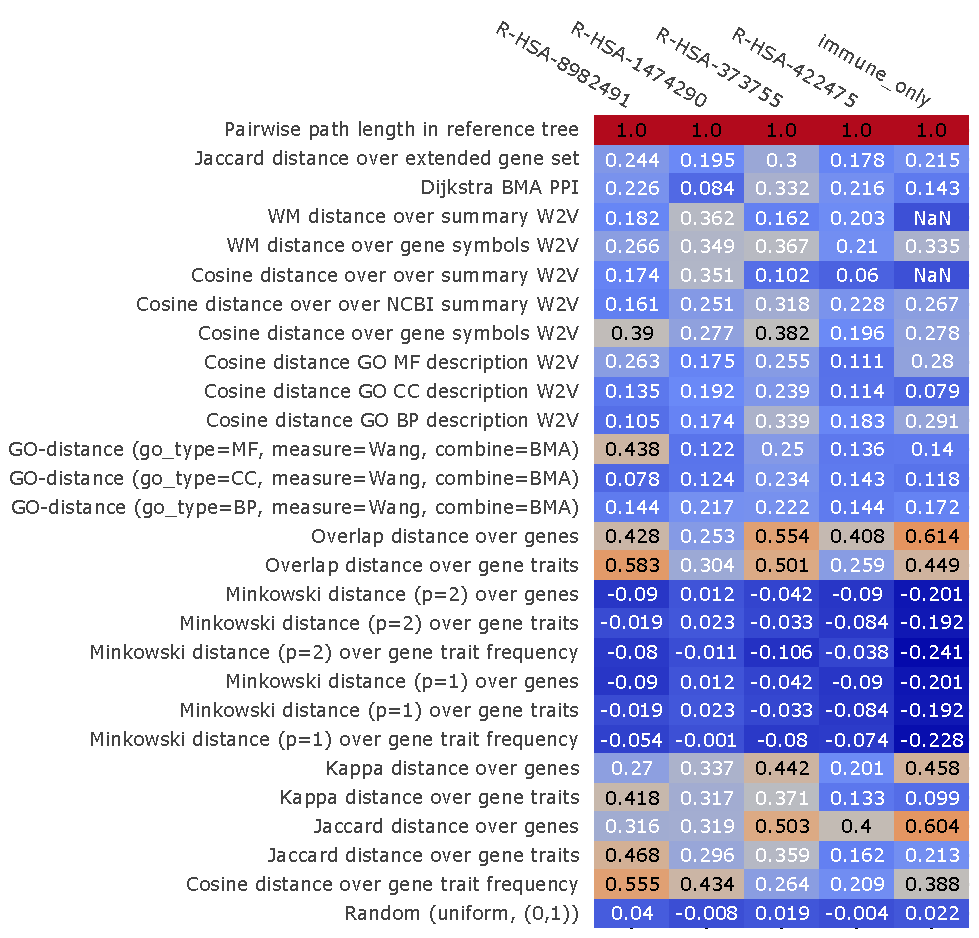
\includegraphics[scale=0.85]{figures/results/plots/summary/spearman.pdf}
	\caption[Spearman correlation between gene set metrics and path lengths]{Spearman correlation between gene set metrics and path lengths. The reason for NaN values in the immune cell dataset is the lack of gene set descriptions from the raw data}
	\label{fig:spearman}
\end{centeredFigure}

We have two possible explanations for the correlation results. 
First, the gene sets from Reactome pathways are always subsets of the gene sets from parent pathways. 
This results in a data-induced bias towards set-based gene set metrics - especially towards the overlap distance. 
This is only partially true for the immune cell reference dataset and the overlap coefficient gives best correlation compared to all other gene set metrics.

Second, we do not consider any uncertainty within the gene sets or the reference trees. 
Even if community-driven curation process insures correctness of the data, it is only a snapshot of the actual biological knowledge base. 
Wrong genes in gene sets or incorrect assignments within in \acrshort{ppi} networks or \acrshort{go} trees could impact the gene set metrics.
This could explain why adding more information (gene descriptions, \acrfull{go} terms) leads to weaker correlation that working only with essential gene set information.

\section{Limitations}

We assume that the biological ground-truth is represented as a rooted tree with gene sets as its nodes. 
Furthermore, we assume that the best way to compare distance metrics with the ground truth is through measuring the correlation between path lengths and metric distances. 
The last assumption is questionable when we compare gene sets that are siblings in the reference trees. 
From a path length perspective, siblings will always have the same distance.
However, every presented gene set metric will assign varying distance values between different pairings of siblings. 
This can lead to incorrect \acrshort{pcc} and \acrshort{srcc}. 
We considered to use distance-based tree-inference algorithm to reconstruct and compare trees from the distance metrics instead.
However, tree-inference algorithm, as they are well established in phylogenetic applications, can only reconstruct dendrograms where no gene set could appear as inner node.
In other words, we would need to sample dendrograms from the reference data sets, which makes it in turn harder to asses the actual usefulness of a gene set metric.

Moreover, we have to mention several technical limitations that comes with the implemented gene set metrics:
\begin{itemize}
	\item The shortest path algorithms like Dijkstra don't consider false nodes or edges between nodes.
	Yu et al. formulate this use-case  as robust shortest path problem, but also prove that this problem is NP-complete~\cite{YU1998457}.
	\item We are not able to execute gene set metrics on \acrshort{wmd} distance if the projected document contains to many vocables (i.e. around $>1000$ vocables). We had to terminate execution as even the pairwise distance calculations took more than one hour to complete. We think that the high time complexity of $O(p^3 \log(p))$, where $p$ is the number of unique vocables,, is the reason for this performance issue. 
	The authors of the \acrshort{wmd} algorithm also propose an optimization that leads to a $O(p^2)$~\cite{KIM2017122}, but this optimization is not part of the Gensim Python package we use.
\end{itemize}

%% ==================
\chapter{Conclusion}
\label{ch:conclusion}
%% ==================

%Recap on your thesis. It has been a long journey if the reader has made it this far. Remind the reader what the big picture was. Briefly outline your thesis, motivation, problem, and proposed solution.

%Now the most important part, draw conclusions based on your analysis. Did your proposed solution work? What are the strong points? What are the limitations?

%Significant issues identified in the thesis, or still outstanding after the thesis, should be describe as future work.

We started this project with the goal to measure differences between gene sets with a biologically plausible gold standard. 
This is the first step in simplifying gene set enrichment analysis, as it often report large lists of gene sets with redundant information.
We introduced a mathematical notation to standardize gene set information and gene set metrics.
Furthermore, we defined and implemented more than 20 gene set metrics by using basic statistical methods, graph-based models, and word embedding models. 
We, moreover, used reference data from Reactome and an immune cell type study to evaluate the gene set metrics. 
We, moreover, downloaded reference data from Reactome and an immune cell type study to evaluate the correlation between metric values and the path lengths in the reference trees. 

Our most important finding is that gene set metrics with more sophisticated models like word embeddings or graphs do not improve the correlation with reference trees.
On the contrary, we get moderate correlation results with statistical methods based on Jaccard index or overlap coefficient that only operate on gene identifiers or phenotype traits. 
Uncertainties in gene sets, reference trees, or models could be an explanation for this observation. 
Adding more information about genes that are wrongly assigned to a gene set could amplify the error in the distance calculation. 
In contrast, we can achieve moderate correlation if we only use phenotype traits instead of more informative gene identifiers. 
The findings, however, assume that a reference tree of gene sets is an appropriate representation of biological plausible distances. 
It is a critical assumption as the manually curated function can contain errors or might does not represent the ground-truth accurately enough.

This leads us to suggest the investigation of in-silico models for gene-centric interactions. 
With in-silico models we can simulate artificial biological systems that mimic simple phenotype traits.
We can use such minimalistic systems as more powerful ground-truth where we sample gene sets randomly or by design.
However, finding a model that approximates biological systems in a computationally feasible way is a difficult question by its own.
The first step is to work on fundamental biochemical network models, which are the main focus of synthetic biology studies~\cite{doi:10.1093/bioinformatics/btg015}. Besides, every ambition to increase quality and reproducibility of published data is always a step forward, as the GIGO-principle applies also for biology and bioinformatics~\cite{Bininda-Emonds2004}.


%We automated these preprocessing steps by using the workflow engine Snakemake~\cite{doi:10.1093/bioinformatics/bts480}. \Cref{fig:reactome_trees} lists all downloaded and preprocessed Reactome subtrees.
% We implemented a Python package that provides \todo{MISSING} gene set metric implementations.
% Use document space based models instead of word space based once

%% ----------------
%% |   Appendix   |
%% ----------------

\cleardoublepage

\appendix

%% ==============================
\chapter{Appendix}
\label{ch:appendix}
%% ==============================

\section{Additional figures}

\begin{centeredFigure}[!ht]
\resizebox{\textwidth}{!}{% <------ Don't forget this %
	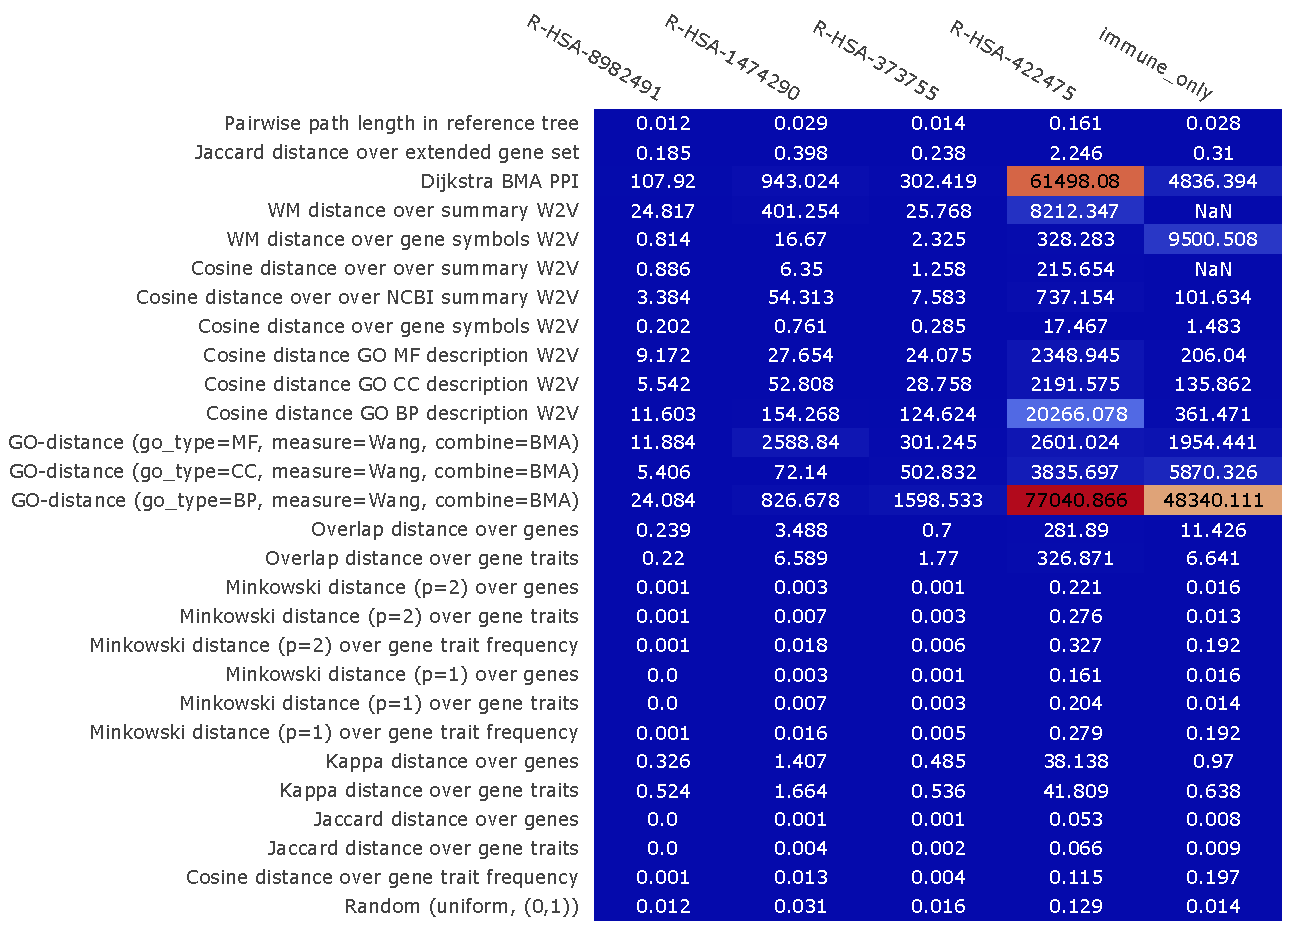
\includegraphics{figures/results/plots/summary/times.pdf}% <------ Don't forget this %
	}
	\caption{Execution time per metric and per entire reference data in seconds}
	\label{fig:times}
\end{centeredFigure}

\begin{centeredFigure}[!ht]
\resizebox{\textwidth}{!}{% <------ Don't forget this %
	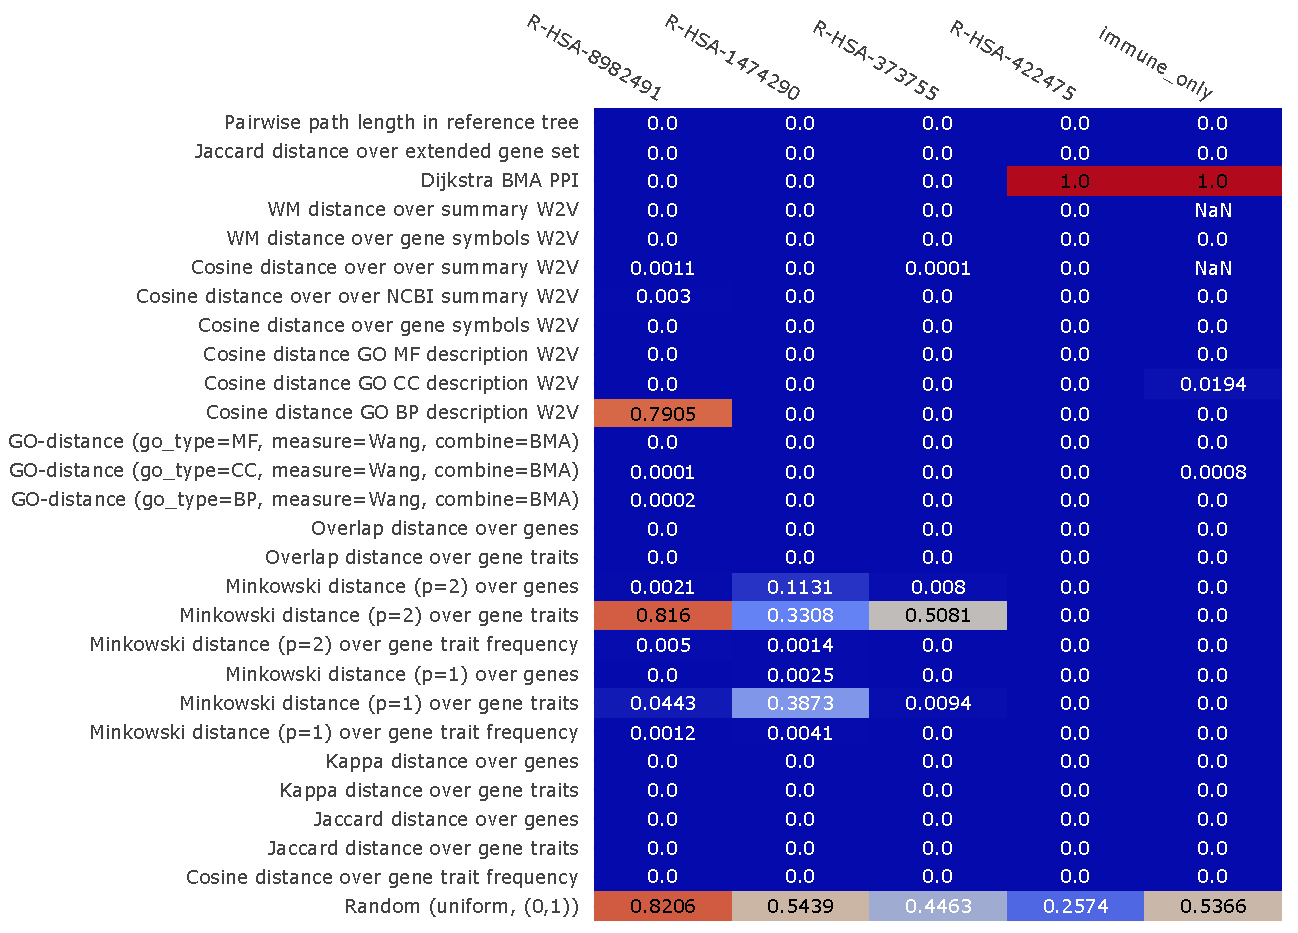
\includegraphics{figures/results/plots/summary/pearsonr_pval.pdf}% <------ Don't forget this %
	}
	\caption{P-values of Pearson correlations coefficients in \cref{fig:pearson}}
	\label{fig:pval_pearson}
\end{centeredFigure}

\begin{centeredFigure}[!ht]
\resizebox{\textwidth}{!}{% <------ Don't forget this %
	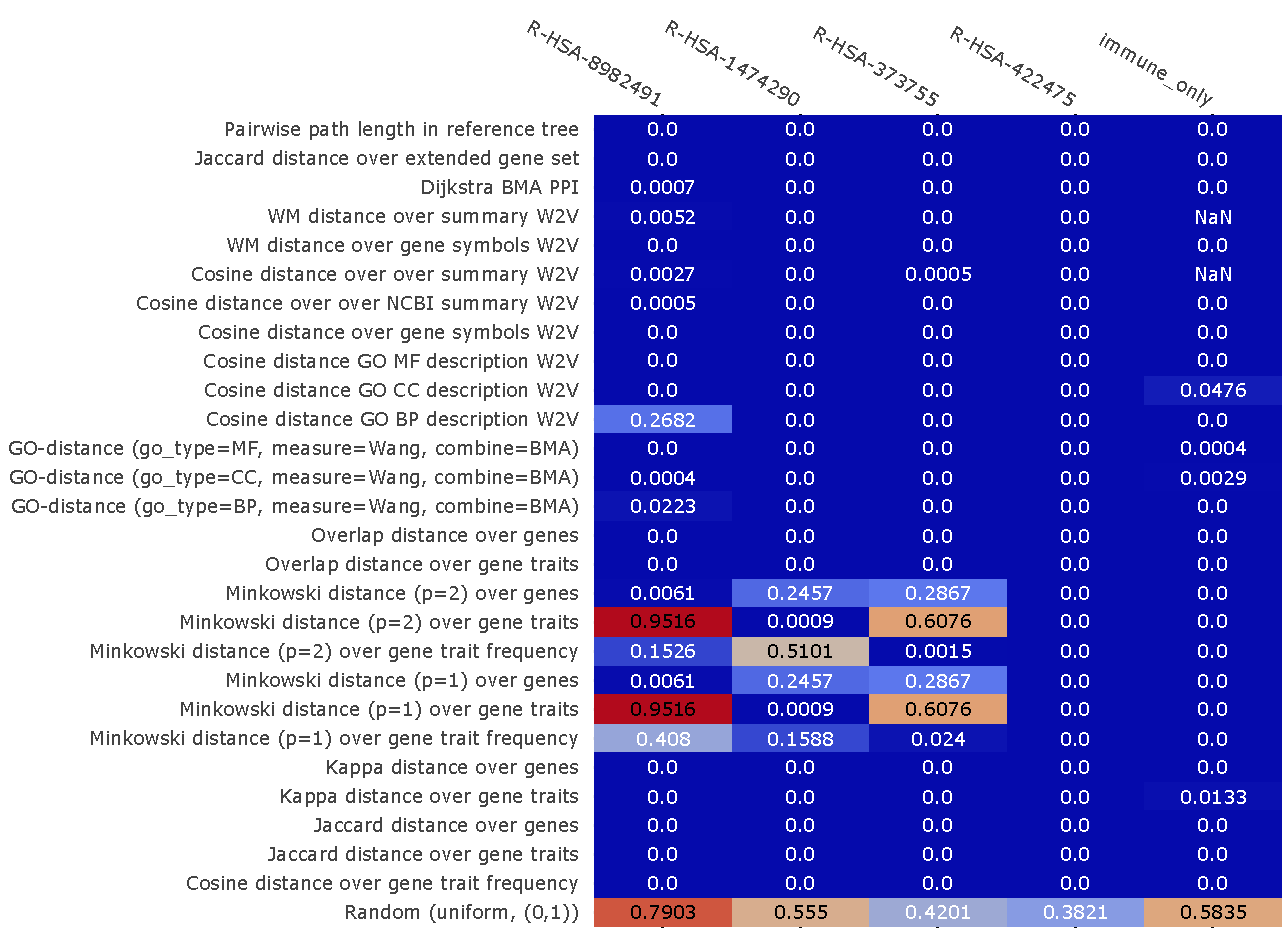
\includegraphics{figures/results/plots/summary/spearmanr_pval.pdf}% <------ Don't forget this %
	}
	\caption{P-values of Spearman's Rank correlations coefficients in \cref{fig:spearman}}
	\label{fig:pval_spearman}
\end{centeredFigure}

\newpage

\global\pdfpageattr\expandafter{\the\pdfpageattr/Rotate 90}
\begin{landscape}
\begin{centeredFigure}[!ht]
	\includegraphics[scale=0.6]{figures/results/plots/full/R-HSA-373755/pearson.pdf}
	\caption{Pearson correlation summary over Reactome dataset R-HSA-373755}
\end{centeredFigure}
\end{landscape}
\global\pdfpageattr\expandafter{\the\pdfpageattr/Rotate 0}

\global\pdfpageattr\expandafter{\the\pdfpageattr/Rotate 90}
\begin{landscape}
\begin{centeredFigure}[!ht]
	\includegraphics[scale=0.6]{figures/results/plots/full/R-HSA-373755/spearman.pdf}
	\caption{Spearman correlation summary over Reactome dataset R-HSA-373755}
\end{centeredFigure}
\end{landscape}
\global\pdfpageattr\expandafter{\the\pdfpageattr/Rotate 0}

\global\pdfpageattr\expandafter{\the\pdfpageattr/Rotate 90}
\begin{landscape}
\begin{centeredFigure}[!ht]
	\includegraphics[scale=0.6]{figures/results/plots/full/R-HSA-1474290/pearson.pdf}
	\caption{Pearson correlation summary over Reactome dataset R-HSA-1474290}
\end{centeredFigure}
\end{landscape}
\global\pdfpageattr\expandafter{\the\pdfpageattr/Rotate 0}

\global\pdfpageattr\expandafter{\the\pdfpageattr/Rotate 90}
\begin{landscape}
\begin{centeredFigure}[!ht]
	\includegraphics[scale=0.6]{figures/results/plots/full/R-HSA-1474290/spearman.pdf}
	\caption{Spearman correlation summary over Reactome dataset R-HSA-1474290}
\end{centeredFigure}
\end{landscape}
\global\pdfpageattr\expandafter{\the\pdfpageattr/Rotate 0}

\global\pdfpageattr\expandafter{\the\pdfpageattr/Rotate 90}
\begin{landscape}
\begin{centeredFigure}[!ht]
	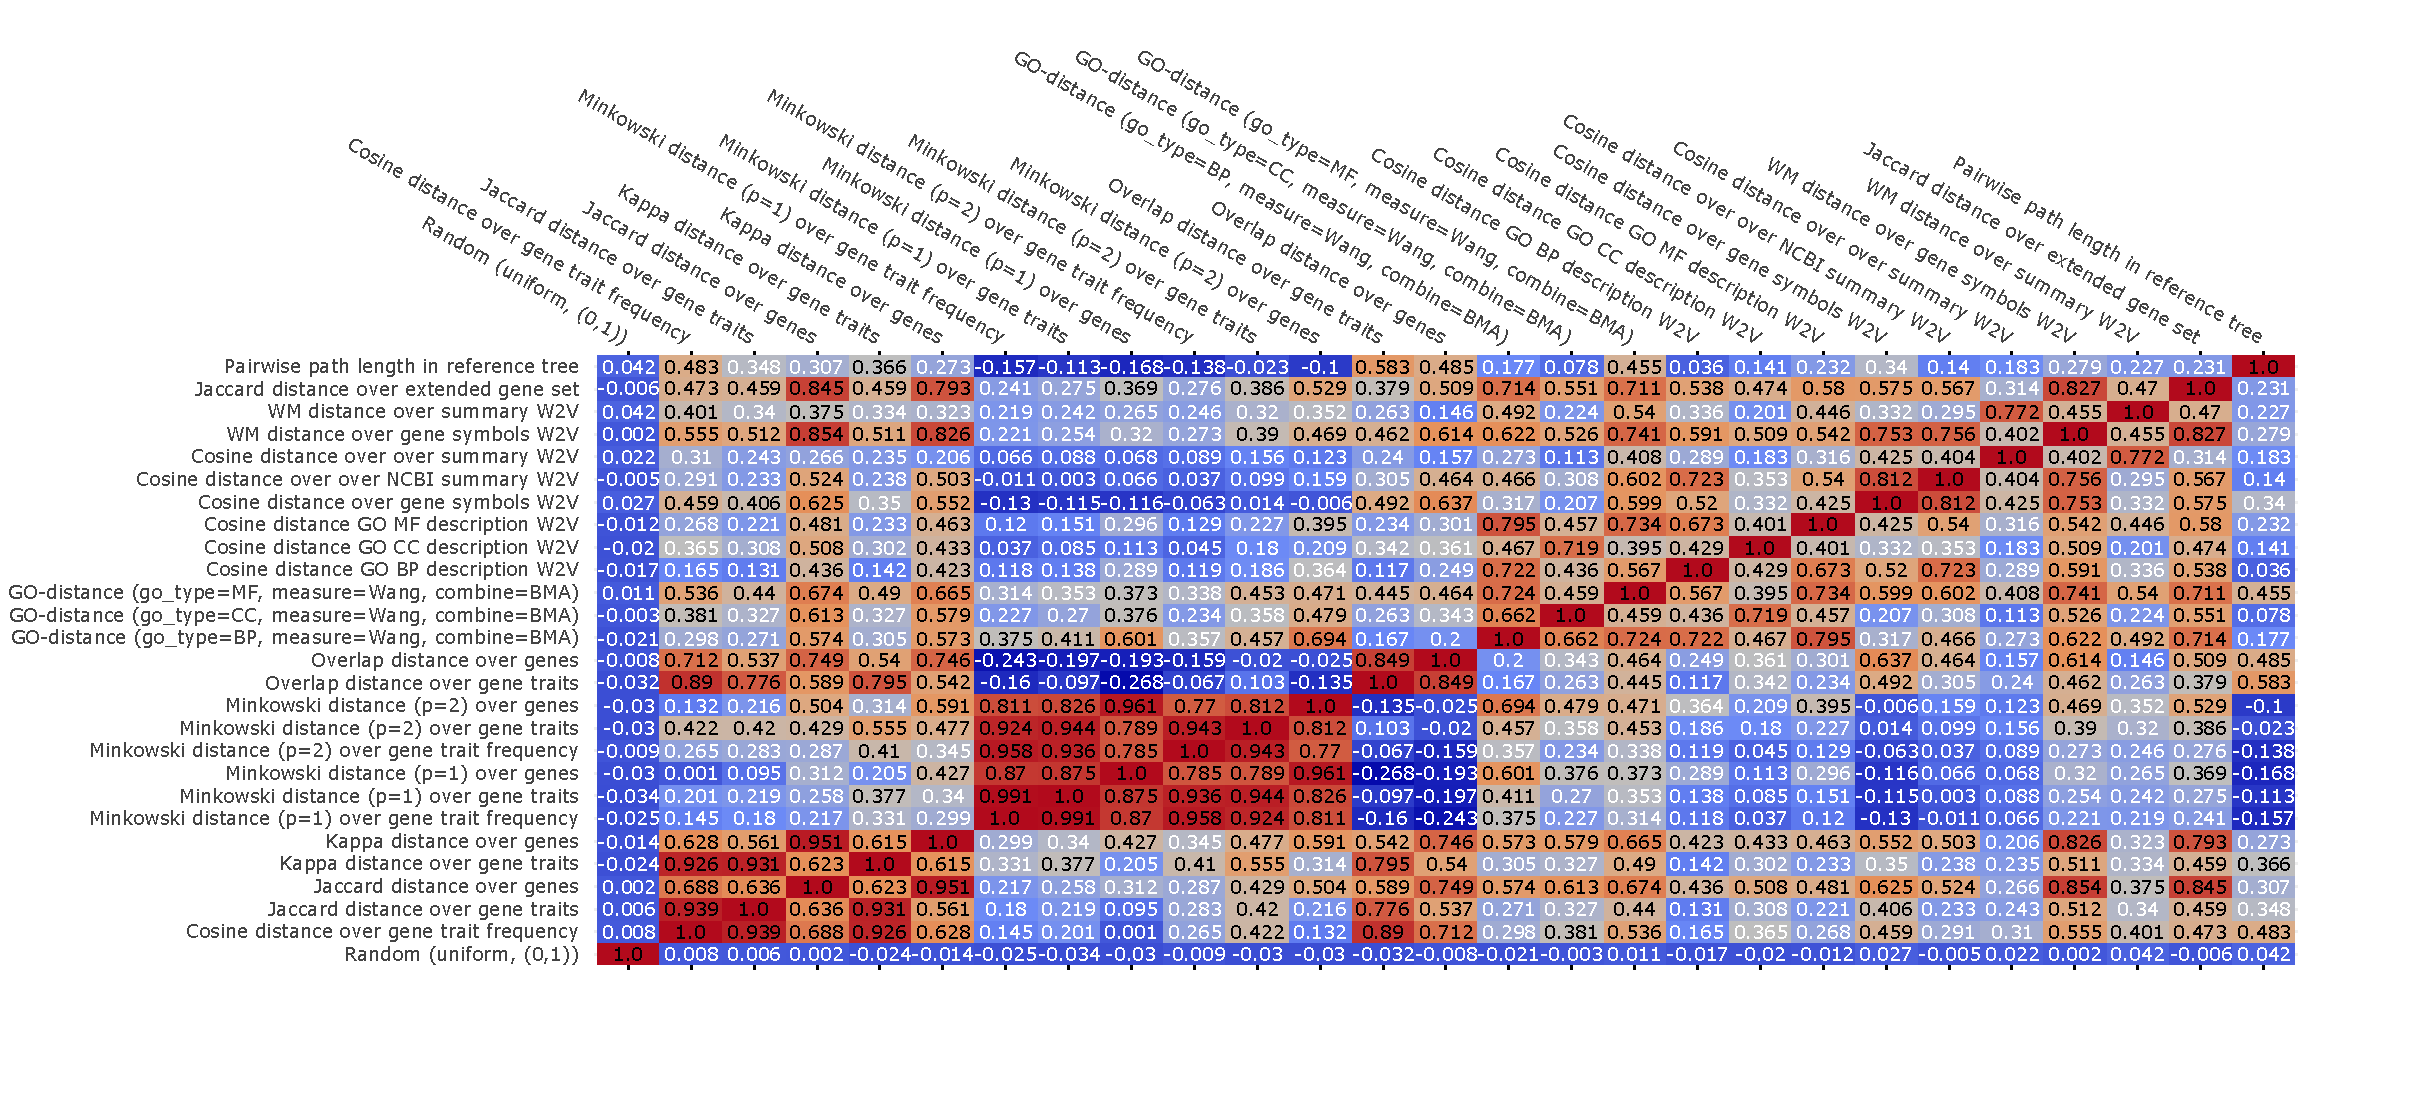
\includegraphics[scale=0.6]{figures/results/plots/full/R-HSA-8982491/pearson.pdf}
	\caption{Pearson correlation summary over Reactome dataset R-HSA-8982491}
\end{centeredFigure}
\end{landscape}
\global\pdfpageattr\expandafter{\the\pdfpageattr/Rotate 0}

\global\pdfpageattr\expandafter{\the\pdfpageattr/Rotate 90}
\begin{landscape}
\begin{centeredFigure}[!ht]
	\includegraphics[scale=0.6]{figures/results/plots/full/R-HSA-8982491/spearman.pdf}
	\caption{Spearman correlation summary over Reactome dataset R-HSA-8982491}
\end{centeredFigure}
\end{landscape}
\global\pdfpageattr\expandafter{\the\pdfpageattr/Rotate 0}

\global\pdfpageattr\expandafter{\the\pdfpageattr/Rotate 90}
\begin{landscape}
\begin{centeredFigure}[!ht]
	\includegraphics[scale=0.6]{figures/results/plots/full/R-HSA-422475/pearson.pdf}
	\caption{Pearson correlation summary over Reactome dataset R-HSA-422475}
\end{centeredFigure}
\end{landscape}
\global\pdfpageattr\expandafter{\the\pdfpageattr/Rotate 0}

\global\pdfpageattr\expandafter{\the\pdfpageattr/Rotate 90}
\begin{landscape}
\begin{centeredFigure}[!ht]
	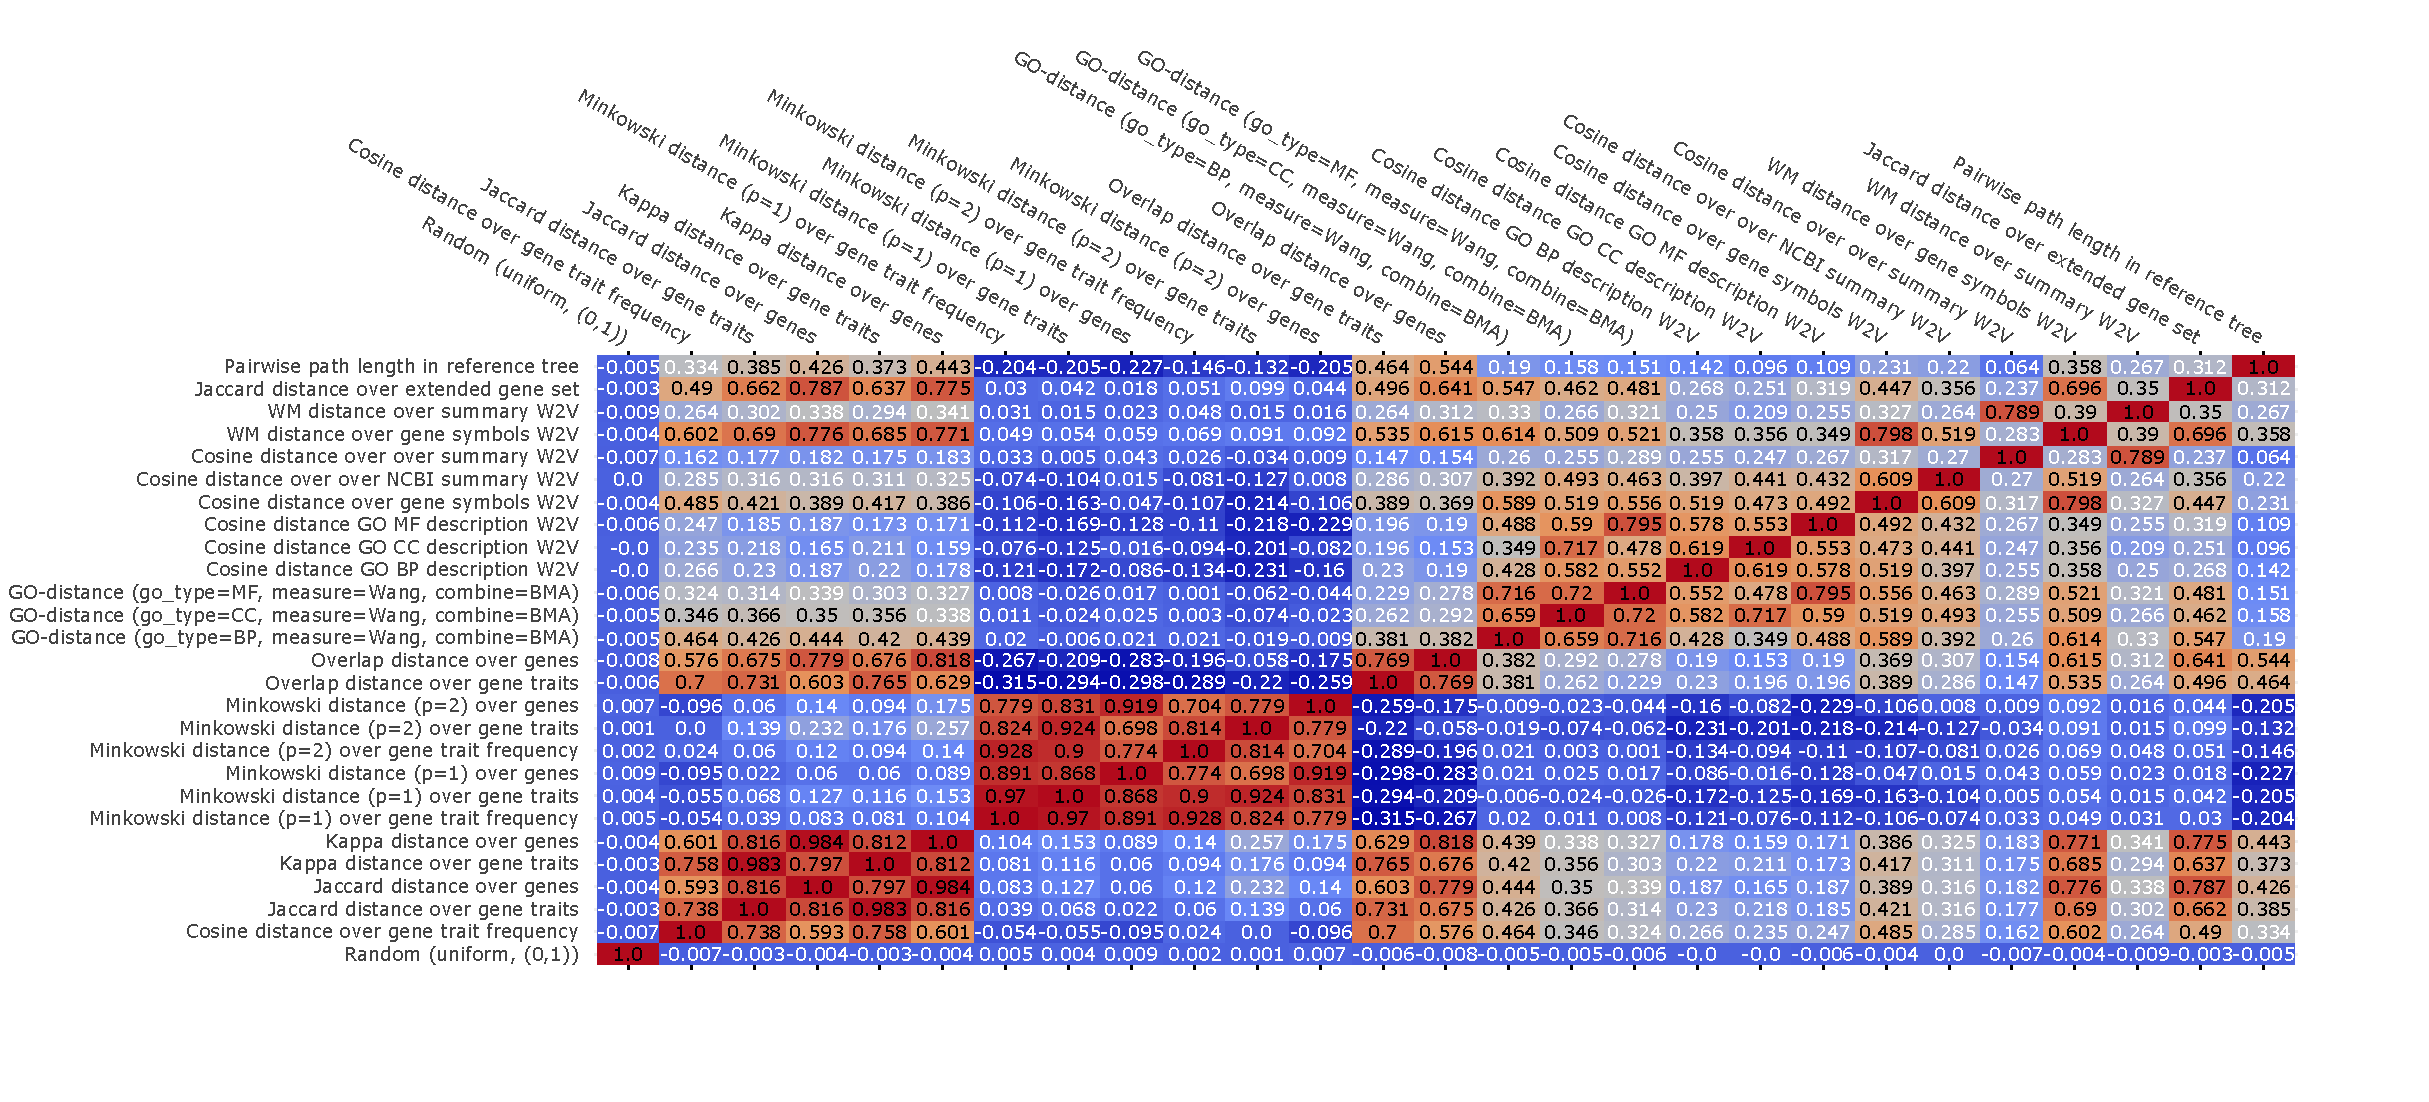
\includegraphics[scale=0.6]{figures/results/plots/full/R-HSA-422475/spearman.pdf}
	\caption{Spearman correlation summary over Reactome dataset R-HSA-422475}
\end{centeredFigure}
\end{landscape}
\global\pdfpageattr\expandafter{\the\pdfpageattr/Rotate 0}

\global\pdfpageattr\expandafter{\the\pdfpageattr/Rotate 90}
\begin{landscape}
\begin{centeredFigure}[!ht]
	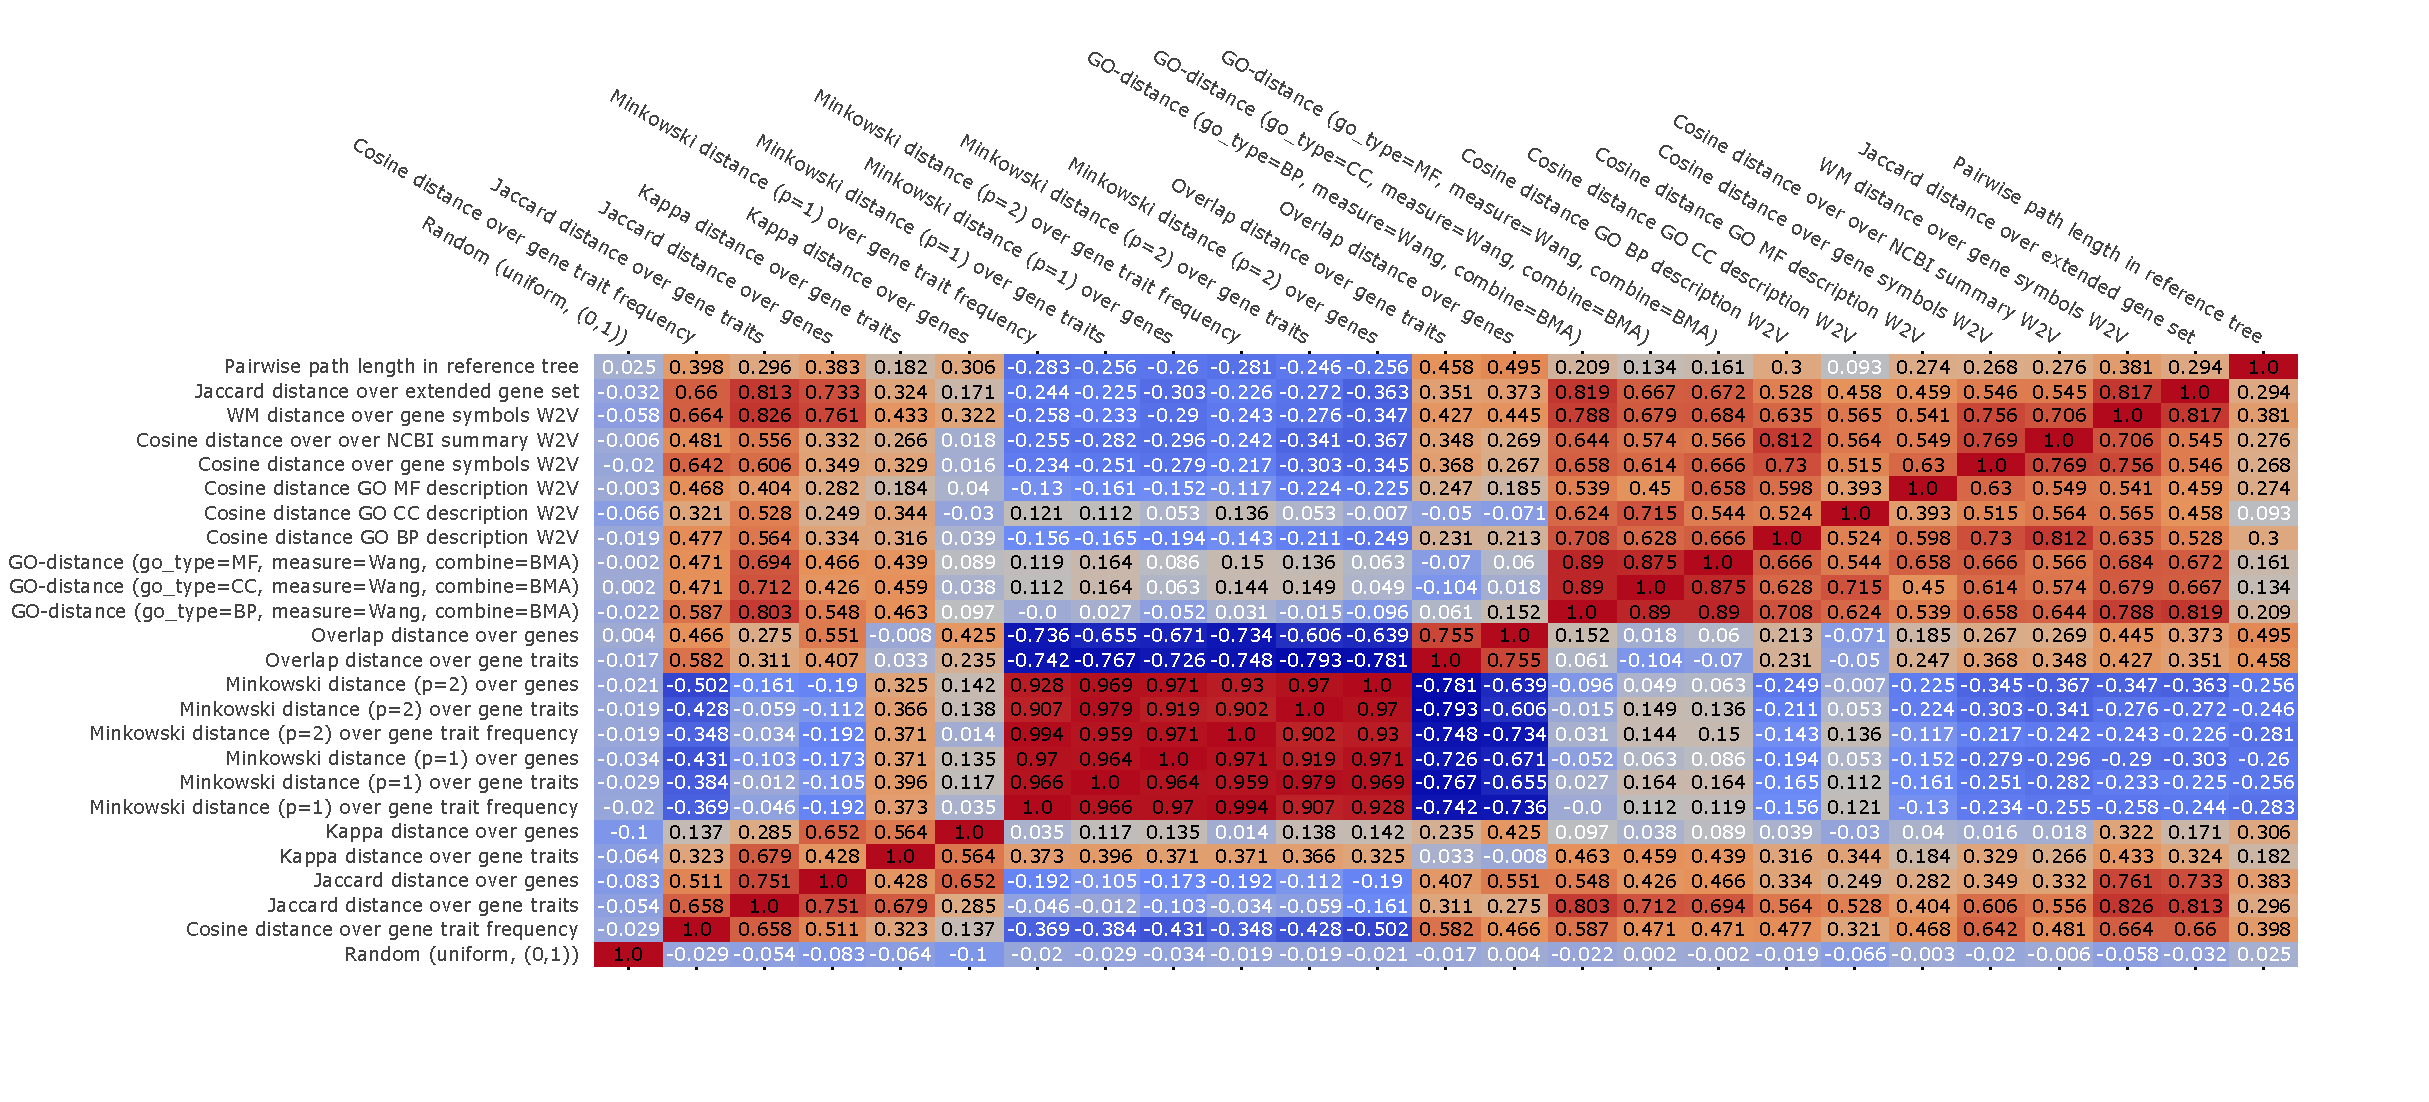
\includegraphics[scale=0.6]{figures/results/plots/full/immune_only/pearson.pdf}
	\caption{Pearson correlation summary over the immune cell reference tree}
\end{centeredFigure}
\end{landscape}
\global\pdfpageattr\expandafter{\the\pdfpageattr/Rotate 0}

\global\pdfpageattr\expandafter{\the\pdfpageattr/Rotate 90}
\begin{landscape}
\begin{centeredFigure}[!ht]
	\includegraphics[scale=0.6]{figures/results/plots/full/immune_only/spearman.pdf}
	\caption{Spearman correlation summary over the immune cell reference tree}
\end{centeredFigure}
\end{landscape}
\global\pdfpageattr\expandafter{\the\pdfpageattr/Rotate 0}

\section{ROGER - Roche Omnibus of Gene Expression Regulation} \label{sec:roger}

\subsection{State of the art}
\subsubsection{Transcriptomic data management}
\subsubsection{Differential Gene Expression Analysis}
\subsubsection{Gene Set Enrichment Analysis}
\subsection{Reimplementation}
\subsubsection{Data structures \& architecture}
\subsubsection{Visualizations \& data access}
 
\newpage 

\section{List of acronyms}
%\setglossarysection{section}
\renewcommand{\glossarysection}[2][]{}
\printglossaries

\section{List of figures}

\listoffigures

\section{List of tables}

\listoftables

\normalsize

%% --------------------
%% |   Bibliography   |
%% --------------------

\cleardoublepage

\iflanguage{english}
{\bibliographystyle{alpha}}
{\bibliographystyle{babalpha-fl}} % german style

\begingroup
\renewcommand{\chapter}[2]{}%
\section{References}
\bibliography{references}
\endgroup


\end{document}
